\subsection{Scenario 1: Requirements prioritisation} \label{val-rp}
The goal of the requirements prioritisation scenario is to validate if the decision design pattern can help software product managers to use evidence-based requirements prioritisation.

\begin{center}
\large\color{document}{\valone} 
\end{center}

A software product manager needs to decide if one requirement is more important than another requirement. The software product manager contributes to reaching the defined goals of the product when the software product manager puts the requirement on the right position in the backlog. These goals are, for example, related to the revenue of the product or the size of its user base. When the software product manager puts the requirement on a higher position in the backlog, then it is supposed to be, another requirement is on a lower position then it should be.

\subsubsection{Decision ontology pattern}
We base the definition of the decision ontology pattern for requirements prioritisation on section \ref{tf-val-rp} \nameref{tf-val-rp} of the theoretical framework. Table \ref{table:rp_formal_dataproperties} presents the knowledge criteria that a software product manager uses to decide which requirement, out of two, is most important. We define the $Requirement$ and $Insight$ (with sub-classes $Challenge$ and $Opportunity$) as decision-relevant \emph{root} classes. We need the $Vision$ class for the reproduction of information. Figure \ref{fig:rpp-ont} presents the ontology.  

\begin{figure}[H]
\centering
  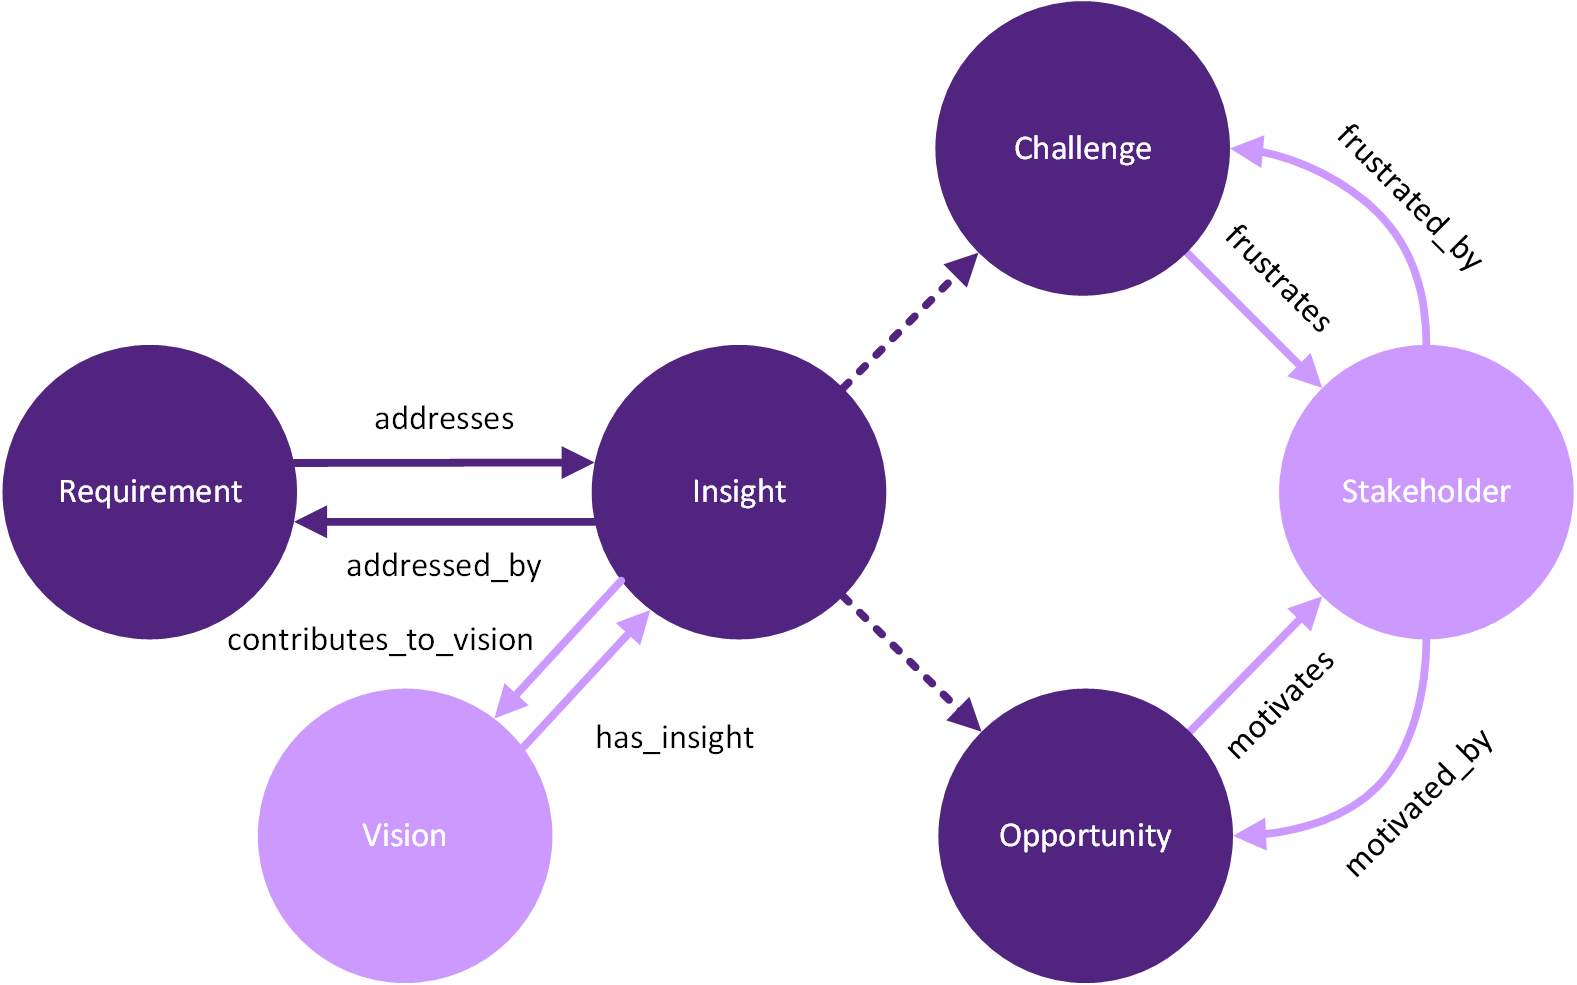
\includegraphics[width=12cm]{../../Images/05_Validation/05_ONT_RP.png}
  \caption{The requirements prioritisation ontology. The \textcolor{Violet}{violet} nodes represent the decision-relevant root classes. The \textcolor{LightViolet}{light violet} nodes represent the classes we need for the reproduction pattern.}
  \label{fig:rpp-ont}
\end{figure}

The $addresses$ and $contribute\_to\_vision$ object properties are essential for the structural integrity of the ontology. A $Requirement$ that does not address an $Insight$ and an $Insight$ that does not contribute to a $Vision$ are structural problems. Missing these object properties influences the reliability of the information that we present in the dashboards.

\subsubsection{Instantiation of the decision ontology pattern}
We instantiate the base decision ontology pattern once for the requirement prioritisation scenario. Code sample \ref{GODP_RP_INST_Basic} presents the instantiation of the base decision ontology pattern. We expand the decision ontology pattern with the ontology figure \ref{fig:rpp-ont} presents manually.

\begin{lstlisting}[float,language=GDOL,caption={The GDOL instantiation code of the basic instantiation of the decision design pattern.},label={GODP_RP_INST_Basic}][H]
Ontology RequirementsPrioritisation = DecisionOntologyPattern_Basic
\end{lstlisting}

The requirements prioritisation ontology and the instantiated decision design pattern include a $Stakeholder$ class. We manually merge the $Stakeholder$ classes from these ontologies into a single $Stakeholder$ class. Alternatively, we could have decided to define both that $Stakeholder$ classes are equal. However, merging the two $Stakeholder$ classes into one class reduces the number of classes and, therefore, reduces the complexity of the ontology.

The context-specific instantiation of the decision design pattern requires parameters to extend the ontology with a context-specific structure. We use the context-specific instantiation to, for example, instantiate the knowledge criteria in a way we can validate their completeness and reproducibility.

Table \ref{table:rp_formal_dataproperties} presents the knowledge criteria that a software product manager needs to understand to decide if one requirement is more important than another requirement. We add the knowledge criteria to the domain of the $Insight$ and $Requirement$ classes of the requirements prioritisation ontology. We define the completeness-level of a $Requirement$ and $Insight$ based on the knowledge criteria. 

\begin{table}[H]
\centering
\caption{An overview of the formal knowledge criteria that requirement prioritisation needs based on the description in section \ref{tf-val-rp} \nameref{tf-val-rp}. Code sample \ref{GODP_RP_INST_Knowledge_Criteria} instantiates the knowledge criteria.}
\begin{tabular}{| p{9cm} | p{4cm} | }
\hline
\rowcolor{document}
\color{documentText}Data Property & \color{documentText}Domain  \\
\hline
$insight\_value$ & $Addressed\_Insight$  \\
\hdashline
$insight\_vision\_contribution$ & $Addressed\_Insight$   \\
\hdashline
$insight\_reach$ & $Addressed\_Insight$  \\
\hdashline
$requirement\_insight\_contribution$ & $Requirement$   \\
\hdashline
$requirement\_value$ & $Requirement$   \\ 
\hdashline
$requirement\_cost$ & $Requirement$   \\ 
\hdashline
$requirement\_confidence$ & $Requirement$  \\ 
\hline
\end{tabular}
\label{table:rp_formal_dataproperties}
\end{table}

We instantiate each knowledge criteria using the generic ontology design pattern presented by code sample \ref{GODP_DDP_Instantiation_Context}. The generic ontology design pattern $DecisionDesignPattern\_Context$ uses two parameters: the information class and the decision-relevant root class. Code sample \ref{GODP_RP_INST_Knowledge_Criteria} presents, for example, the instantiation of the $insight\_value$ as an example. Code sample \ref{GODP_RP_INST_Knowledge_Criteria_Result} shows the instantiated generic ontology design pattern.

\begin{lstlisting}[float,language=GDOL,caption={The GDOL instantiation code of the knowledge criteria.},label={GODP_RP_INST_Knowledge_Criteria}][H]
DecisionOntologyPattern_Context[insight_value][Addressed_Insight]
\end{lstlisting}

\begin{lstlisting}[float,language=GDOL,caption={The result of the GDOL instantiation code that code sample \ref{GODP_RP_INST_Knowledge_Criteria} presents.},label={GODP_RP_INST_Knowledge_Criteria_Result}][H]
Completeness_op [has_information_insight_value][Addressed_Insight][insight_value] 
\end{lstlisting}

Code sample \ref{SHACL_RP_INST_Completeness} shows the instantiated SHACL shapes for, for example, the $insight\_value$. We need to adjust the $sh:targetClass$, $sh:path$, and $sh:message$ variables manually.

The constraints generate three violations when a knowledge criterion is not available. One violation represents the unavailability of the knowledge criterion itself, and the other two violations represent the missing $data\_value$ and $data\_description$. It is possible to add more violations if the context requires this.

\begin{lstlisting}[float,language=SHACL,caption={An example of instantiated SHACL shapes for the data property $insight\_value$. We instantiate this code sample for each knowledge criterion and for each information required to reproduce a knowledge criterion.},label={SHACL_RP_INST_Completeness}][H]
rp:Addressed_InsightShape a sh:NodeShape;
	sh:targetClass rp:Addressed_Insight; 
	sh:property [
		sh:path rp:has_information_insight_value;
		sh:severity sh:Violation; 
		sh:minCount 1; 
		sh:message "Completeness: add insight_value to the Addressed_Insight."; ];
	sh:property [
		sh:path rp:has_information_insight_value;
		sh:severity sh:Violation; 
		sh:minCount 1; 
		sh:message "Completeness: add data_value to the insight_value."; ];
	sh:property [
		sh:path rp:has_information_insight_value;
		sh:severity sh:Violation; 
		sh:minCount 1; 
		sh:message "Completeness: add data_description to the insight_value."; ];
\end{lstlisting}

The reproduction of knowledge criteria uses the completeness pattern. With the instantiation of the generic ontology design pattern and the constraints, we can validate the reproducibility of the knowledge criteria throughout the information chain figure \ref{fig:reproducibility_chain_val_rp} shows.

\begin{figure}[H]
\centering
  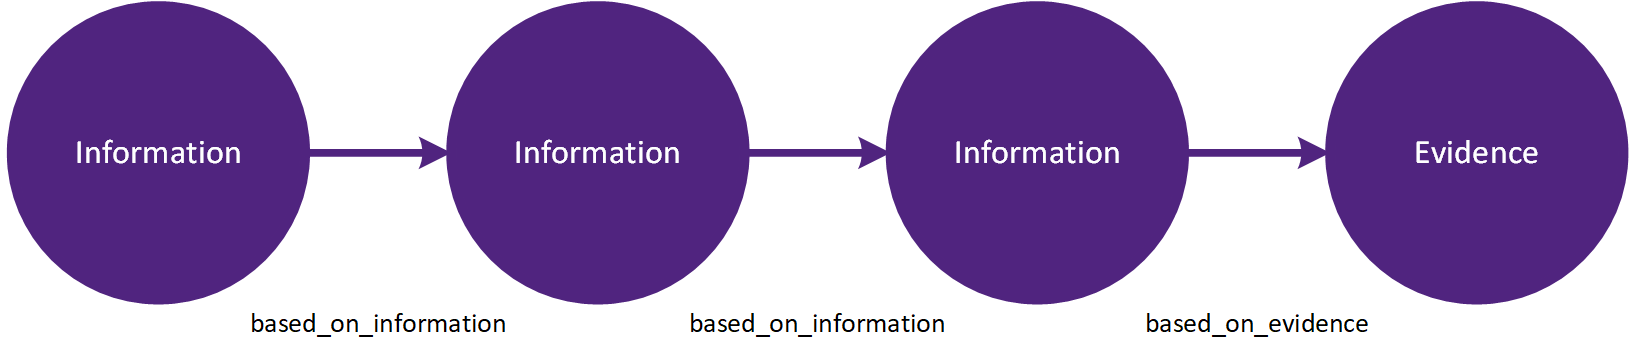
\includegraphics[width=12cm]{../../Images/Reproducibility_Chain.png}
  \caption{An example of an evidence-based chain of information. The reproducibility pattern should detect if the chain is not evidence-based.}
  \label{fig:reproducibility_chain_val_rp}
\end{figure} 

\paragraph{Insight value}
The insight value takes input from the stakeholder on the \emph{frustration} (challenge) or \emph{motivation} (opportunity) the stakeholder experiences. We consider a description of the \emph{business case} from the stakeholder's perspective as well. Table \ref{table:rpp_insight_value} presents an overview of the background information the software product manager requires to define the insight value.

\begin{table}[H]
\centering
\caption{The background information that we require to reproduce the value of an insight.}
\begin{tabular}{| p{3cm} | p{4cm} | p{8cm} | }
\hline
\rowcolor{document}
\color{documentText}$has\_in{\f}ormation\_*$ & \color{documentText}Class & \color{documentText}Description  \\
\hline
$challenge\_$ ${\f}rustration$ & $Addressed\_Challenge$ & The current pain the stakeholder experiences. A stakeholder finds this insight a necessary \emph{fix}. \\
\hdashline
$opportunity\_$ $motivation$ & $Addressed\_Opportunity$ & The motivation of a stakeholder to use the product more often if a requirement addresses this insight. \\
\hdashline
$insight\_$ $business\_case$ & $Addressed\_Insight$ & Increased revenue, decreased cost, or decreased business risk. \\
\hline
\end{tabular}
\label{table:rpp_insight_value}
\end{table}

Code sample \ref{GDOP_RP_INST_Insight_Value} presents the instantiation of the $Insight\_Value$. 

\begin{lstlisting}[float,language=GDOL,caption={The GDOL instantiation code of the information reproducing the $Insight\_Value$},label={GDOP_RP_INST_Insight_Value}][H]
DecisionDesignPattern_Context[challenge_frustration; Addressed_Challenge]
DecisionDesignPattern_Context[opportunity_motivation; Addressed_Opportunity] 
DecisionDesignPattern_Context[insight_business_case; Addressed_Insight]
\end{lstlisting}

\paragraph{Vision contribution}
The vision itself needs to be defined to validate if the insight contributes to the vision. We introduce the $Vision$ class for this. The vision class hosts the vision statement (and related time frame), a measurable objective (and related time frame), a current state and target condition. Table \ref{table:rp_vision_contribution} presents an overview of the background information the software product manager requires to define the vision contribution. 

\begin{table}[H]
\centering
\caption{The background information that we require to reproduce the vision contribution of an insight.}
\begin{tabular}{| p{3cm} | p{2cm} | p{10cm} | }
\hline
\rowcolor{document}
\color{documentText}$has\_in{\f}ormation\_*$ & \color{documentText}Class & \color{documentText}Description  \\
\hline
$vision\_$ $statement$ & $Used\_Vision$ & A futuristic goal defined in the context of a product or company. \\ 
\hdashline
$vision\_measureable\_$ $objective$ & $Used\_Vision$ & A description of a measurable objective that achieves the first step towards a futuristic goal. \\ 
\hdashline
$vision\_target\_ $ $condition$ & $Used\_Vision$ & The first smaller objective that contributes to achieving a measurable objective. \\ 
\hdashline
$vision\_current\_ $ $state$ & $Used\_Vision$ & A description of today's status related to the target condition. \\ 
\hline
\end{tabular}
\label{table:rp_vision_contribution}
\end{table}

We can reproduce the $Insight\_Vision\_Contribution$ based on data properties stored in an $Insight$ and $Vision$. The domain of the $Insight\_Vision\_Contribution$ itself is an $Insight$. 

Code sample \ref{GDOP_RP_INST_Vision_Contribution} presents the instantiation of the $Insight\_Vision\_Contribution$. 

\begin{lstlisting}[float,language=GDOL,caption={The GDOL instantiation code of the information reproducing the $Insight\_Vision\_Contribution$},label={GDOP_RP_INST_Vision_Contribution}][H]
DecisionDesignPattern_Context[vision_statement; Used_Vision] 
DecisionDesignPattern_Context[vision_measurable_objective; Used_Vision]
DecisionDesignPattern_Context[vision_target_condition; Used_Vision]
DecisionDesignPattern_Context[vision_current_state; Used_Vision]
\end{lstlisting}

Additionally, code sample \ref{GDOP_RP_INST_Vision_Contribution_Time_Frame} presents the instantiation code to validate that the time frame of the vision statement and the time frame of the measurable objective are complete. Validating the completeness of the time frames is outside of the scope of the decision design pattern as these are very context-specific. Therefore, we use the instantiation of the completeness pattern directly.

\begin{lstlisting}[float,language=GDOL,caption={The GDOL instantiation code of the time frames of the $vision\_measurable\_objective$ and the $vision\_statement$.},label={GDOP_RP_INST_Vision_Contribution_Time_Frame}][H]
Completeness_dp[time_frame; vision_measurable_objective; xsd:dateTime] 
Completeness_dp[time_frame; vision_statement; xsd:dateTime] 
\end{lstlisting}

The default constraints cover the missing information, the related $data\_value$, and $data\_description$. Missing decision-relevant information typically results in three violations. In this case, we need to add the $time\_{\f}rame$ to the $vision\_measurable\_objective$ and the $vision\_statement$ and generate four violations. Therefore, we add two additional constraints to the $VisionShape$. Code sample \ref{SHACL_RP_INST_time_frame} presents these two additional constraints.

\begin{lstlisting}[float,language=SHACL,caption={The SHACL shapes that validate the completeness of the $time\_{\f}rame$ data property in the context of the vision statement and the measurable objective.},label={SHACL_RP_INST_time_frame}][H]
sh:property [
	sh:path rp:has_information_vision_statement;
	sh:severity sh:Violation; 
	sh:minCount 1; 
	sh:message "Completeness: add time_frame to the vision_statement."; ];
sh:property [
	sh:path rp:has_information_vision_measurable_objective;
	sh:severity sh:Violation; 
	sh:minCount 1; 
	sh:message "Completeness: add time_frame to the vision_measurable_objective."; ];
\end{lstlisting}

\paragraph{Insight reach}
Figure \ref{fig:rpp-ont} presents an ontology that allows multiple stakeholders to raise their frustration or motivation towards a specific insight. Ideally, each stakeholder is represented in the ontology as an individual and connected to an $Insight$ using the $motivates$ or ${\f}rustrates$ object properties. In this case, we can easily calculate the $insight\_reach$ by taking the percentage of stakeholders, out of the total pool of stakeholders that are frustrated or motivated by the insight. Table \ref{table:rpp_insight_reach} presents an overview of the background information the software product manager requires to define the insight reach. 

\begin{table}[H]
\centering
\caption{The background information that we require to reproduce the reach of an insight.}
\begin{tabular}{| p{5cm} | p{2cm} | p{8cm} | }
\hline
\rowcolor{document}
\color{documentText}Object property & \color{documentText}Domain & \color{documentText}Range  \\
\hline
$motivates$ & $Opportunity$ & $Stakeholder$ \\ 
\hdashline
${\f}rustrates$ & $Challenge$ & $Stakeholder$ \\ 
\hline
\end{tabular}
\label{table:rpp_insight_reach}
\end{table}

Code sample \ref{GDOP_RP_INST_Insight_Reach} presents the instantiation of the $Insight\_Vision\_Contribution$. In this case, we create a direct link between the requirements prioritisation ontology and the reproducibility pattern. Therefore, we use the instantiation of the completeness pattern. However, it is nearly impossible to get all of the stakeholders registered and capture their specific insights. Alternatively, we base the $insight\_reach$ on, for example, evaluated external evidence. In this case, the $insight\_reach$ should be reproducible by evidence. 

\begin{lstlisting}[float,language=GDOL,caption={The instantiation of the completeness pattern that contributes to the reproducibility of the $insight\_value$.},label={GDOP_RP_INST_Insight_Reach}][H]
Completeness_op[motivates; Addressed_Opportunity; Stakeholder] 
Completeness_op[frustrates; Addressed_Challenge; Stakeholder] 
\end{lstlisting}

\paragraph{Requirement cost}
The cost of the requirement depends on the time it takes to implement the requirement, the cost of purchasing equipment\footnote{The cost of purchasing equipment can be based on, for example, a quotation classified as validated external evidence.}, and the cost of gaining knowledge that is required to realise the requirement. The team that defines this information implements the requirement as well. Table \ref{table:rpp_requirement_cost} presents an overview of the background information the software product manager requires to define the requirement cost.

\begin{table}[H]
\centering
\caption{The background information that we require to reproduce the cost of a requirement.}
\begin{tabular}{| p{3cm} | p{2.5cm} | p{9.5cm} | }
\hline
\rowcolor{document}
\color{documentText}$has\_in{\f}ormation\_*$ & \color{documentText}Class & \color{documentText}Description  \\
\hline
$requirement\_$ $knowledge\_cost$ & $Requirement$ & The estimated total cost to acquire knowledge that allows the team to implement the requirement. \\ 
\hdashline
$requirement\_$ $equipment\_cost$ & $Requirement$ & The estimated total purchasing costs of the equipment needed to implement the requirement. The cost can include, for example, processing hardware, sensors, and software licenses. \\ 
\hdashline
$requirement\_size$ & $Requirement$ & The estimated size of the requirement. The estimated size is a relative value, and its range depends on the way of working of the team. \\ 
\hline
\end{tabular}
\label{table:rpp_requirement_cost}
\end{table}

Code sample \ref{GDOP_RP_INST_Requirement_Cost} presents the instantiation of the $Requirement\_Cost$. 

\begin{lstlisting}[float,language=GDOL,caption={The GDOL instantiation code of the information reproducing the $Requirement\_Cost$},label={GDOP_RP_INST_Requirement_Cost}][H]
DecisionDesignPattern_Context[requirement_knowledge_cost; Requirement] 
DecisionDesignPattern_Context[requirement_equipement_cost; Requirement]
DecisionDesignPattern_Context[requirement_size; Requirement]
\end{lstlisting}

\paragraph{Requirement value}
The $insight\_value$ represents the value of the insight for the stakeholder. The $requirement\_value$ represents the value of the requirement for the organisation developing the requirement. The requirement value typically ranges from an opportunity to increase revenue, decrease costs, or decrease certain risks. Table \ref{table:rpp_requirement_value} presents an overview of the background information the software product manager requires to define the value of the requirement.

\begin{table}[H]
\centering
\caption{The background information that we require to reproduce the value of a requirement.}
\begin{tabular}{| p{3cm} | p{2.5cm} | p{9.5cm} | }
\hline
\rowcolor{document}
\color{documentText}$has\_in{\f}ormation\_*$ & \color{documentText}Class & \color{documentText}Description  \\
\hline
$requirement\_$ $increase\_revenue$ & $Requirement$ & The description of how this requirement increases the revenue of the organisation developing the requirement. \\ 
\hdashline
$requirement\_$ $decrease\_cost$ & $Requirement$ & The description of how this requirement decreases the costs (or increases the efficiency) of the organisation developing the requirement. \\ 
\hdashline
$requirement\_$ $decrease\_risk$ & $Requirement$ & The description of how this requirement decreases a particular risk the organisation faces. \\ 
\hline
\end{tabular}
\label{table:rpp_requirement_value}
\end{table}

Code sample \ref{GDOP_RP_INST_Requirement_Value} presents the instantiation of the $Requirement\_Cost$. 

\begin{lstlisting}[float,language=GDOL,caption={The GDOL instantiation code of the information reproducing the $Requirement\_Value$},label={GDOP_RP_INST_Requirement_Value}][H]
DecisionDesignPattern_Context[requirement_increase_revenue; Requirement] 
DecisionDesignPattern_Context[requirement_decrease_cost; Requirement]
DecisionDesignPattern_Context[requirement_decrease_risk; Requirement]
\end{lstlisting}

\paragraph{Insight contribution}
A product manager can address one insight using different requirements. The team that addresses the insight can slice the insight into various requirements. The requirement contribution to an opportunity depends on the motivation we can spark with the requirement. Alternatively, the $requirement\_contribution$ to the challenge depends on the frustration we can take away using the requirement. Table \ref{table:rpp_insight_contribution} presents an overview of the background information the software product manager requires to define the insight contribution.

\begin{table}[H]
\centering
\caption{The background information that we require to reproduce the insight contribution of a requirement.}
\begin{tabular}{| p{4cm} | p{4cm} | p{7cm} | }
\hline
\rowcolor{document}
\color{documentText}$has\_in{\f}ormation\_*$ & \color{documentText}Class & \color{documentText}Description  \\
\hline
$challenge\_{\f}rustration$ & $Addressed\_Challenge$ & The frustration we can take away by implementing the requirement. \\ 
\hdashline
$opportunity\_motivation$ & $Addressed\_Opportunity$ & The motivation we can spark by implementing the requirement. \\ 
\hline
\end{tabular}
\label{table:rpp_insight_contribution}
\end{table}

Code sample \ref{GDOP_RP_INST_Requirement_Contribution} presents the instantiation of the $Requirement\_Insight\_Contribution$. We ensure that challenges that are addressed by an insight have a challenge, and opportunities that are addressed by a requirement have a motivation.

\begin{lstlisting}[float,language=GDOL,caption={The GDOL instantiation code of the information reproducing the $Requirement\_Insight\_Contribution$},label={GDOP_RP_INST_Requirement_Contribution}][H]
DecisionDesignPattern_Context[challenge_frustration; Addressed_Challenge]
DecisionDesignPattern_Context[motivation_opportunity; Addressed_Opportunity]
\end{lstlisting}

\paragraph{Requirement confidence}
The requirement confidence represents the confidence of the team that implements the requirement. The team is aware that a larger requirement is more time consuming to implement than a smaller requirement. Teams that need to acquire a lot of knowledge might be less confident compared to teams that already have most of the knowledge to realise the requirement. Table \ref{table:rpp_requirement_confidence} presents an overview of the background information the software product manager requires to define the requirement confidence. We instantiated the $requirement\_knowledge\_cost$ and $requirement\_size$ in the context of the $requirement\_cost$.

\begin{table}[H]
\centering
\caption{The background information that we require to reproduce the cost of a requirement.}
\begin{tabular}{| p{3cm} | p{2.5cm} | p{9.5cm} | }
\hline
\rowcolor{document}
\color{documentText}$has\_in{\f}ormation\_*$ & \color{documentText}Class & \color{documentText}Description  \\
\hline
$requirement\_$ $knowledge\_cost$ & $Requirement$ & The estimated total cost to acquire knowledge that allows the team to realise the requirement. \\ 
\hdashline
$requirement\_size$ & $Requirement$ & The estimated size is a relative value, and its range depends on the way of working of the team. \\ 
\hline
\end{tabular}
\label{table:rpp_requirement_confidence}
\end{table}

\paragraph{Instantiation overview}
We combine the requirements prioritisation ontology and the decision ontology pattern. Additionally, we instantiate a new class for each information type, for example, the $Requirement\_Size$. The new information types are sub-classes of the $In{\f}ormation$ root classes. The decision ontology pattern validates that the individuals classified as $In{\f}ormation$ and the information types that are subclasses of $In{\f}ormation$ are evidence-based. Figure \ref{fig:05_RP_Instantiated} presents a conceptual overview of the instantiation. We have summarized the information types in three main information classes: $Vision\_*$ includes the information classes related to the vision, $Requirement\_*$ includes the information classes related to the requirement, and $Insight\_*$ includes the information classes related to the insight. 

\begin{figure}[H]
\centering
  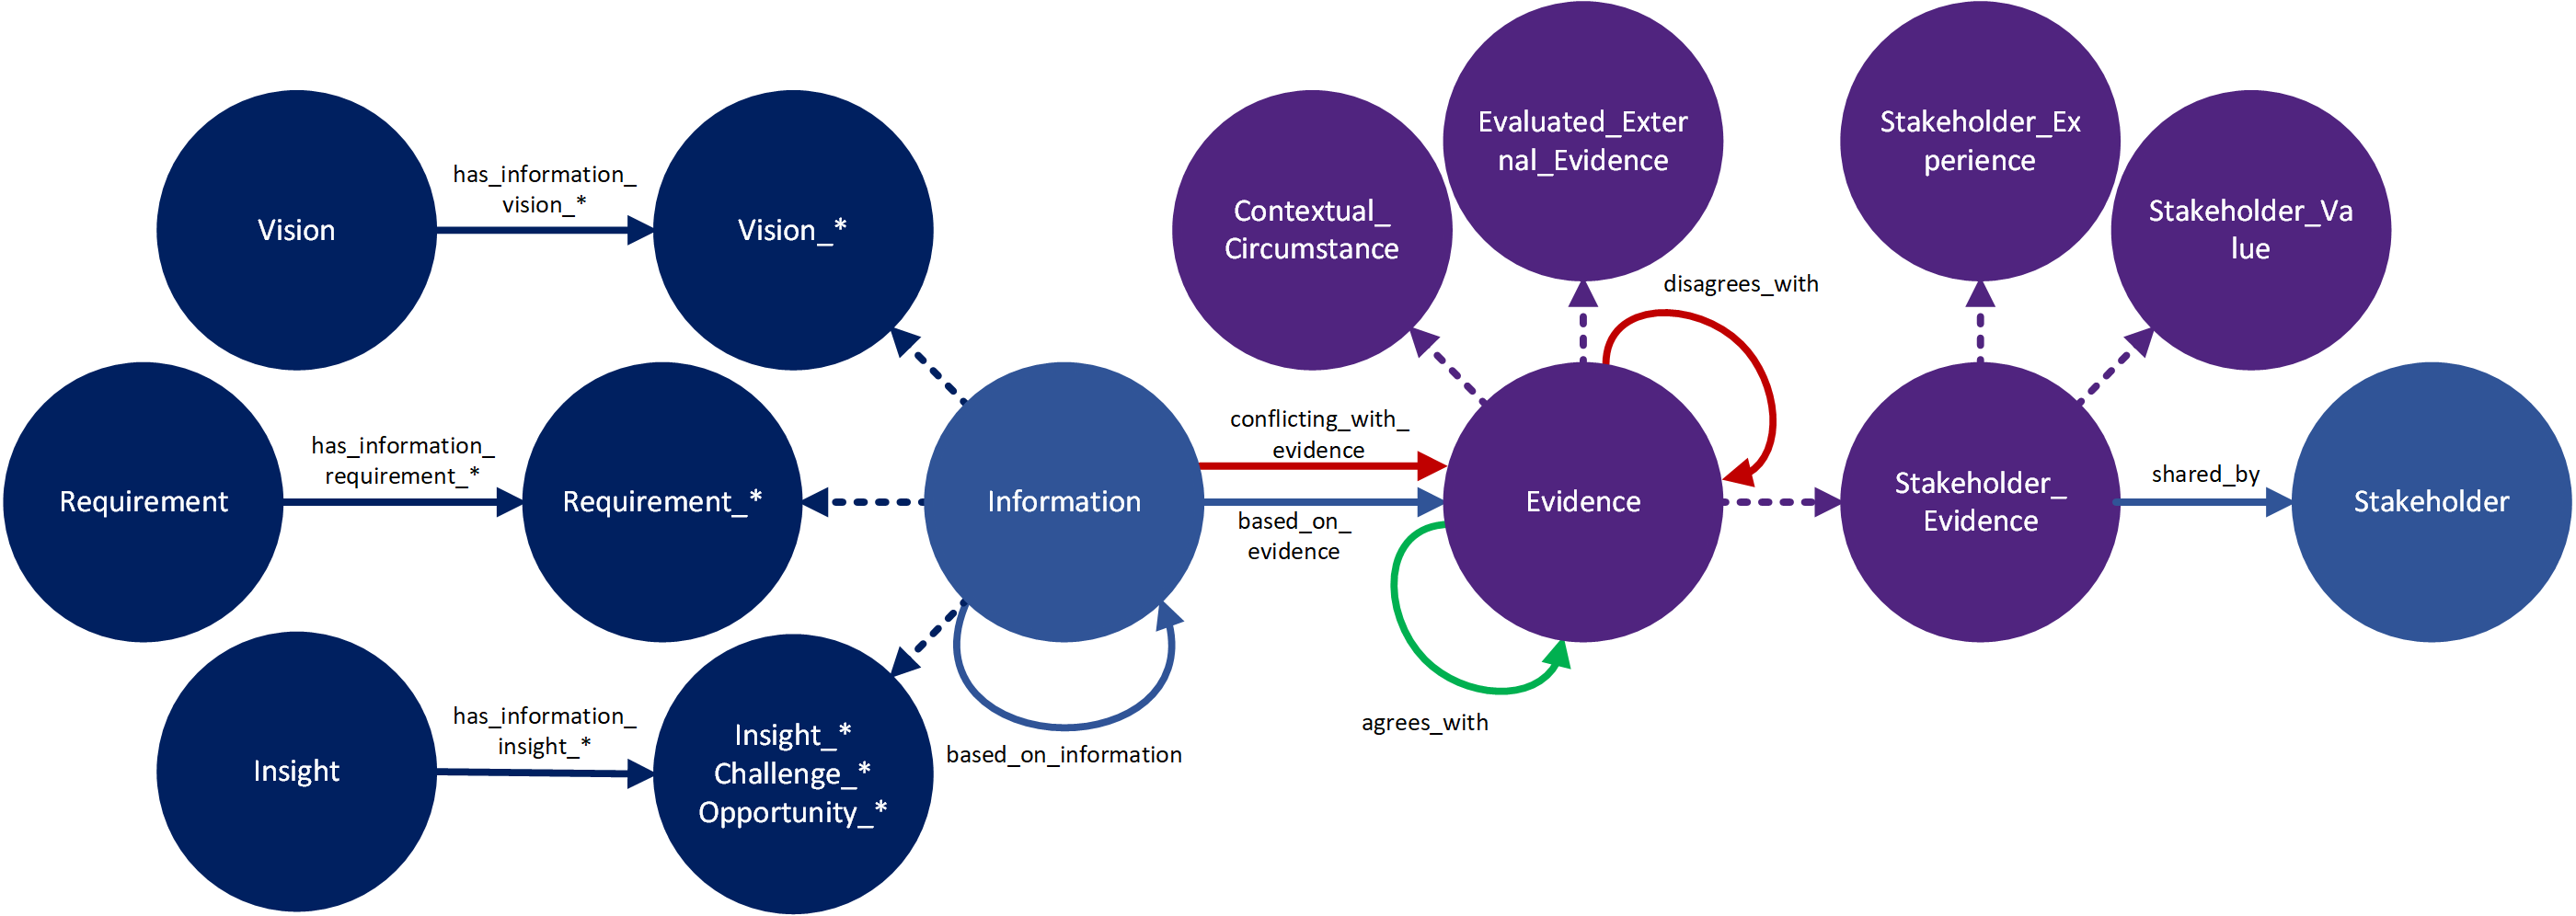
\includegraphics[width=17cm]{../../Images/05_Validation/05_RP_Instantiated.png}
  \caption{The combined requirements prioritisation ontology and the decision design pattern ontology.}
  \label{fig:05_RP_Instantiated}
\end{figure}

\subsubsection{Structural validation}
An incorrect maximum number of violations can cause an incorrect information maturity-level. The structural violations are not part of the functions that define the information maturity-level. Two scenarios can cause an incorrect maximum number of violations:
\begin{enumerate}
\item A requirement does not address an insight. In this case, we cannot retrieve the maximum number of violations for the insight.
\item An insight does not contribute to a vision. In this case, we cannot retrieve the maximum number of violations for the vision.
\end{enumerate}

While the reasoner finds structural violations, the dashboards are not reliable and will not show up. The decision-maker needs to solve the structural violations first.

\paragraph{Structural validation: $Insight$ contributes to $Vision$}
We add the object properties $has\_insight$, $contributes\_to\_vision$, and $in{\f}ormation\_of$ (including the sub-object properties $in{\f}ormation\_of\_requirement$, $in{\f}ormation\_of\_vision$, and $in{\f}ormation\_of\_insight$) to detect the visions that have an $Insight$. The $in{\f}ormation\_of$ object property (and its sub-object properties) are the inverse of the $has\_in{\f}ormation$ object property (and its sub-object properties). The reasoner infers the $contributes\_to\_vision$ object property from the super property figure \ref{fig:05_RP_contributes_to_vision_SP} presents. $has\_insight$ is the inverse of $contributes\_to\_vision$. 

\begin{figure}[H]
\centering
  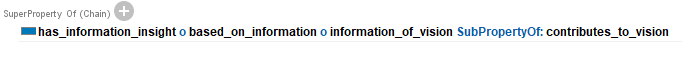
\includegraphics[width=17cm]{../../Images/05_Validation/05_RP_Contributes_To_Vision_SP.png}
  \caption{The Prot\'eg\'e configuration of the super property that the reasoner uses to infer the $contributes\_to\_vision$ object property.}
  \label{fig:05_RP_contributes_to_vision_SP}
\end{figure}

Figure \ref{fig:05_RP_contributes_to_vision} presents the super property that infers the $contributes\_to\_vision$ and $has\_insight$ object properties automatically if we can trace an $Insight$ to a $Vision$ using the chain of object properties.

\begin{figure}[H]
\centering
  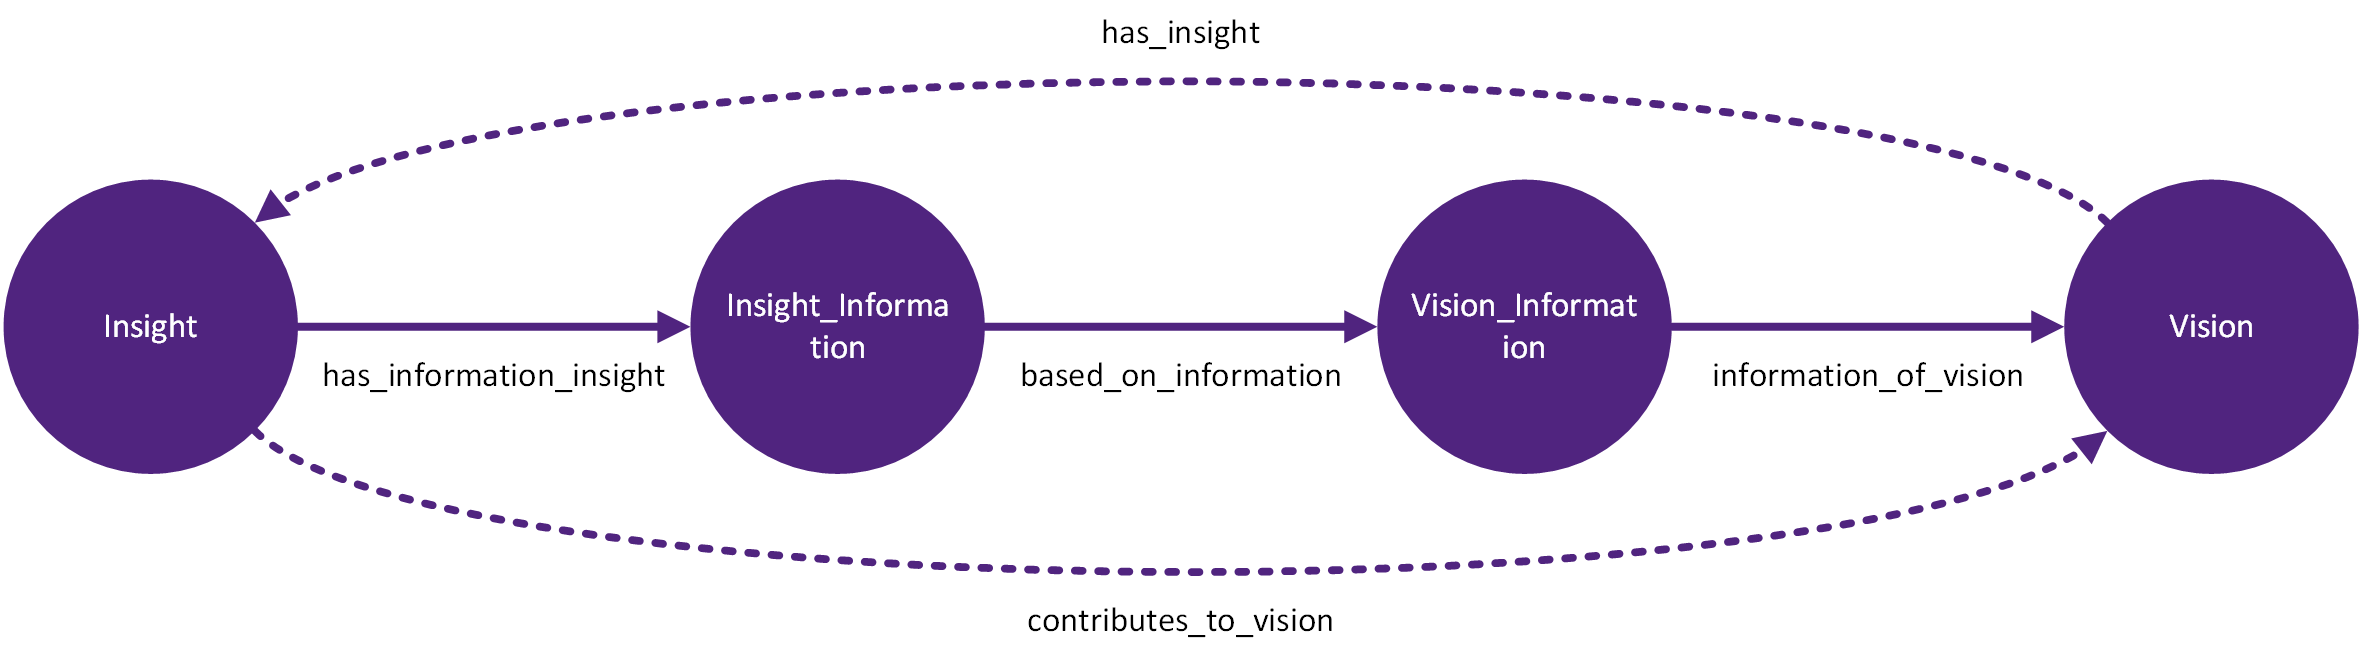
\includegraphics[width=17cm]{../../Images/05_Validation/05_RP_Contributes_To_Vision.png}
  \caption{The super property infers the $contributes\_to\_vision$ and $has\_insight$ object properties automatically if there is a trace from an $Insight$ to a $Vision$ using the chain of object properties. The reasoner infers the dotted lines using the super property.}
  \label{fig:05_RP_contributes_to_vision}
\end{figure}

Code sample \ref{SHACL_RP_STRUC_INSVIS} presents the SHACL shapes we use to detect that an $Insight$ does not contribute to a $Vision$. Without the super property figure \ref{fig:05_RP_contributes_to_vision} presents the constraints would need to validate three object properties on three target classes. In this case, the super property enables the reasoner to infer these three object properties into a single object property. This example shows that inferencing reduces the complexity of the constraints. 

\begin{lstlisting}[float,language=SHACL,caption={The SHACL shapes we use to detect that an $Addressed\_Insight$ does not contribute to a $Vision$.},label={SHACL_RP_STRUC_INSVIS}][H]
rp:Addressed_InsightShape a sh:NodeShape;
	sh:targetClass rp:Addressed_Insight; 
	sh:property [
		sh:path rp:contributes_to_vision;
		sh:severity sh:Violation;
		sh:minCount 1;
		sh:message "Structural: Insight does not contribute to a Vision." ; ];
\end{lstlisting}

\paragraph{Structural validation: $Requirement$ addresses $Insight$}
We want the software product manager to focus on the relevant individuals. Therefore, the constraints should only generate violations for individuals that are relevant for a decision. For example, we need to prevent that an $Insight$ that is not addressed by a $Requirement$ generates a violation. This $Insight$ is not relevant yet. However, the constraints should generate a violation as soon as a $Requirement$ addresses this $Insight$.

First, we use the $Addressed\_Insight$ sub-class to identify the insights that a requirement addresses. Insights that a requirement does not address are not relevant for requirements prioritisation. We use the same concept for the $Addressed\_Opportunity$ and the $ Addressed\_Challenge$. The $Addressed\_Opportunity$ and the $Addressed\_Challenge$ are subclasses of the $Addressed\_Insight$ as well. 

We also want to make sure every requirement that a software product manager prioritises addresses an insight. The reasoner infers the $addresses$ object property from the super property figure \ref{fig:05_RP_Addresses} presents.

\begin{figure}[H]
\centering
  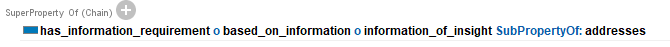
\includegraphics[width=17cm]{../../Images/05_Validation/05_RP_Addresses.png}
  \caption{The Prot\'eg\'e configuration of the super property that the reasoner uses to infer the $contributes\_to\_vision$ object property.}
  \label{fig:05_RP_Addresses}
\end{figure}

Figure \ref{fig:addressed_requirement} presents the super property that infers the $addresses$ object property automatically if we can trace a $Requirement$ to an $Insight$ using the chain of object properties.

\begin{figure}[H]
\centering
  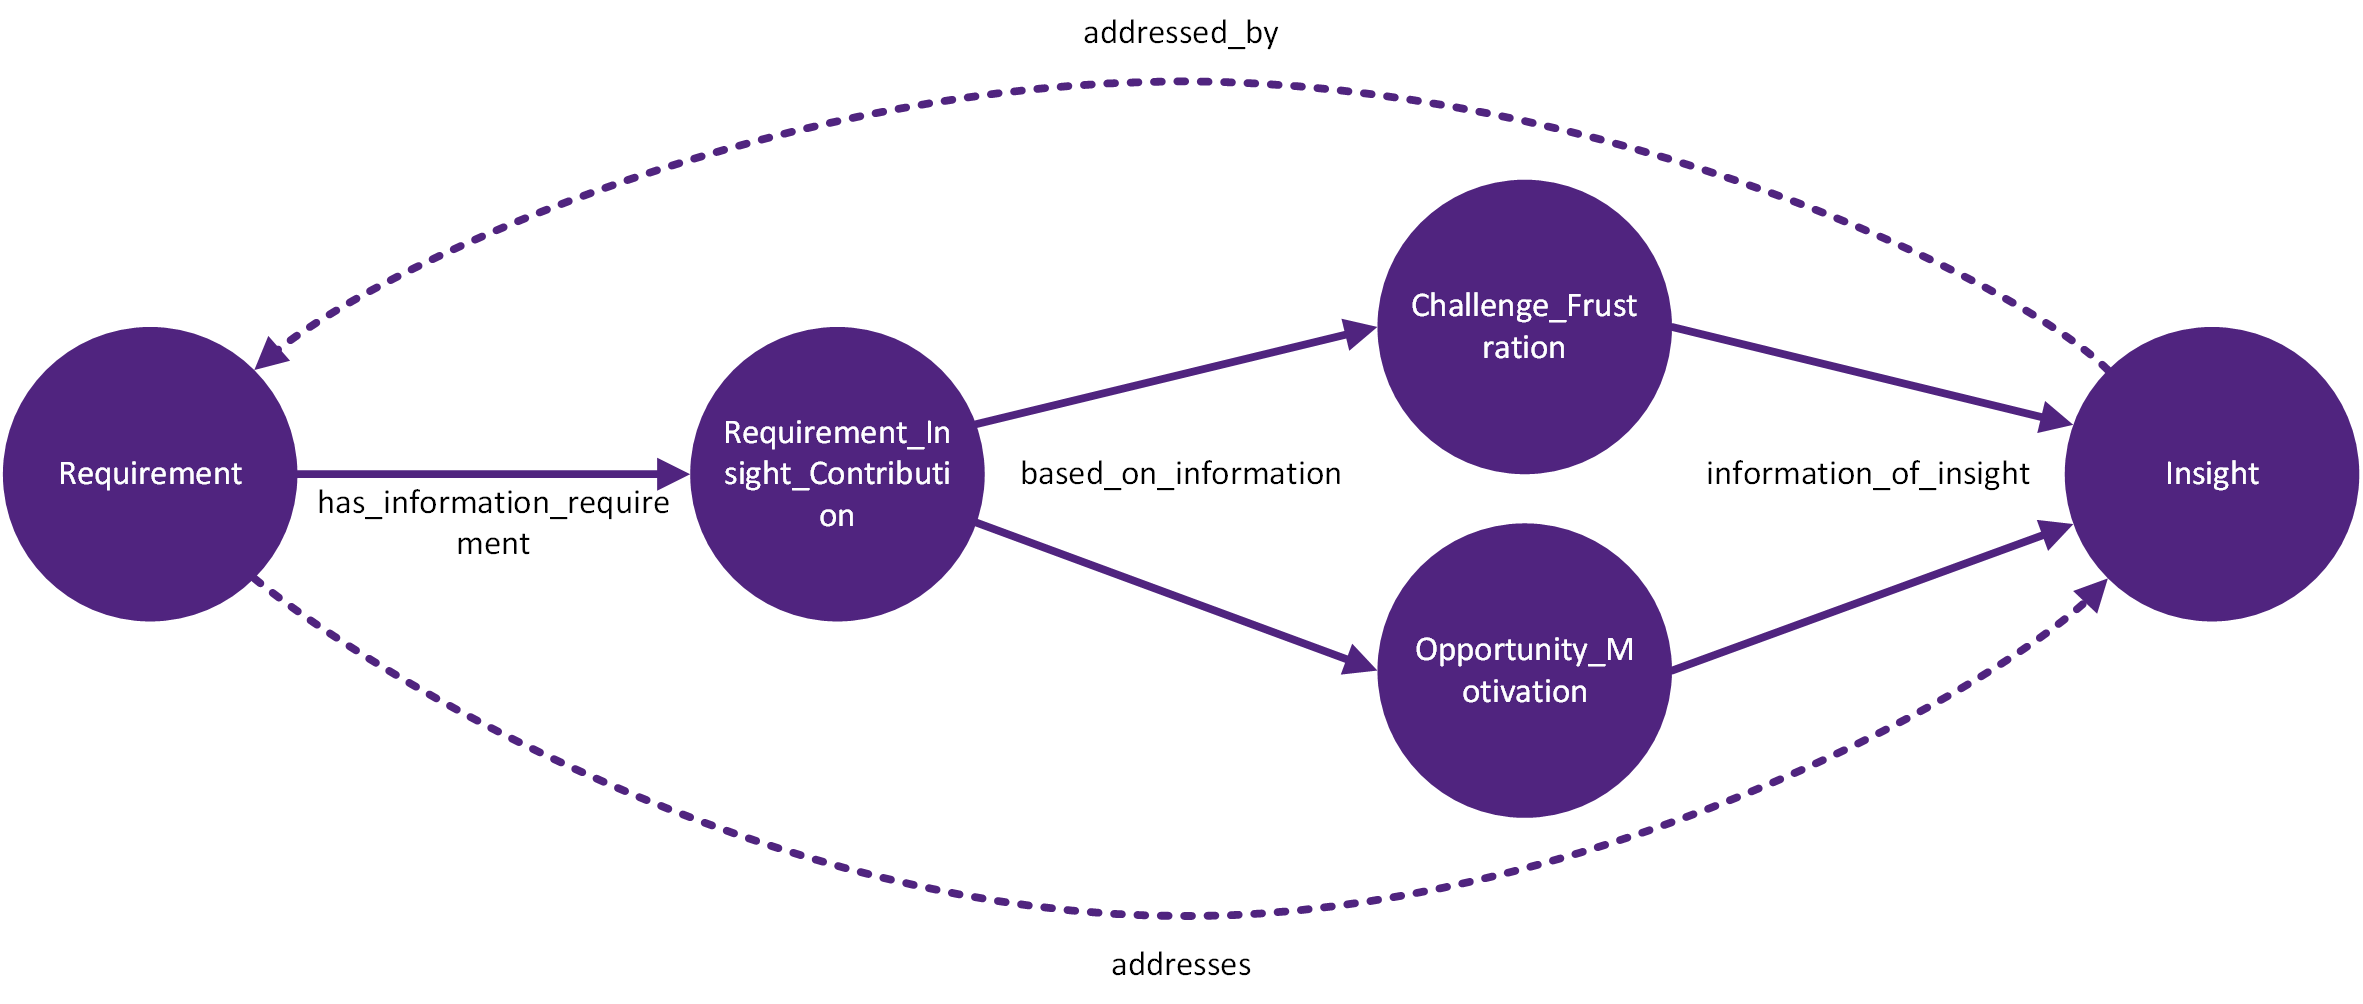
\includegraphics[width=15cm]{../../Images/05_Validation/05_RP_Addresses_Overview.png}
  \caption{The super property that infers the $addresses$ object property automatically if we can trace a $Requirement$ to an $Insight$ using the chain of object properties.}
  \label{fig:addressed_requirement}
\end{figure}

Code sample \ref{SHACL_RP_STRUC_ADD} presents the SHACL shapes we use to detect that a $Requirement$ does not address an $Insight$.

\begin{lstlisting}[float,language=SHACL,caption={The SHACL shapes we use to detect that a $Requirement$ does not address an $Insight$.},label={SHACL_RP_STRUC_ADD}][H]
rp:RequirementShape a sh:NodeShape;
	sh:targetClass rp:Requirement; 
	sh:property [
		sh:path rp:addresses; 
		sh:severity sh:Violation; 
		sh:minCount 1; 
		sh:message "Structural: Requirement does not address an Insight."; 
\end{lstlisting}

\subsubsection{Test scenarios for the decision ontology pattern}
We define six abstract test scenarios. The abstraction makes it easier to validate that a specific scenario triggers the expected violations. Scenario $SC0$ validates the structure of the ontology. The first scenario ($SC1$) should not generate any violations. The other scenarios validate a specific pattern and are structurally valid. This structure limits the complexity of the scenarios and their outcomes. 

\paragraph{Scenario 0 ($SC0$): Structural validation}
The requirements, insights, and visions we use in the other scenarios are structurally valid. Each $Requirement$ addresses at least one $Insight$, and each $Insight$ contributes to at least one $Vision$. We create $Requirement\_SC0$ for this. $Requirement\_SC00$ does not address an $Insight$ and should generate one structural violation and one reproducibility violation. $Requirement\_SC00\_Insight\_Contribution$ generates the reproducibility violation as we did not base it on the motivation of frustration of an insight. This missing link breaks the chain figure \ref{fig:addressed_requirement} presents and generates the structural violation. Figure \ref{fig:RP_SC0_Requirement_SC00_Insight_Contribution} presents the configuration of $Requirement\_SC00\_Insight\_Contribution$ in Prot\'eg\'e.

\begin{figure}[H]
\centering
  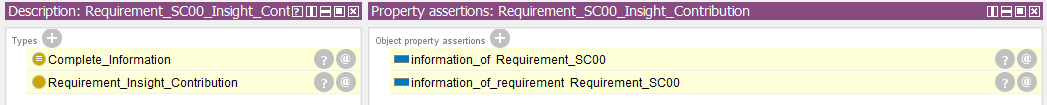
\includegraphics[width=17cm]{../../Images/05_Validation/05_RP_Requirement_SC00_Insight_Contribution.png}
  \caption{The individual $Requirement\_SC00\_Insight\_Contribution$ in Prot\'eg\'e. The $in{\f}ormation\_o{\f}$ object property is the inverse of the $has\_in{\f}ormation$ object property. The reasoner uses this characteristic to infer the $in{\f}ormation\_o{\f}$ object property. }
  \label{fig:RP_SC0_Requirement_SC00_Insight_Contribution}
\end{figure}

Additionally, we define $Requirement\_SC01$. $Requirement\_SC01$ addresses $Opportunity\_SC01$. Therefore $Requirement\_SC01$ should not trigger a structural violation. However, $Opportunity\_SC01$ does not contribute to a $Vision$. $Opportunity\_SC01$ should generate one structural validation and one reproducibility violation. $Opportunity\_SC01\_Vision\_Contribution$ generates the reproducibility violations as we did not base it on vision relevant information. This missing link breaks the chain figure \ref{fig:05_RP_contributes_to_vision} presents and generates the structural violation. Figure \ref{fig:RP_SC0_Opportunity_SC01_Vision_Contribution} presents the configuration of $Opportunity\_SC01\_Vision\_Contribution$ in Prot\'eg\'e.

\begin{figure}[H]
\centering
  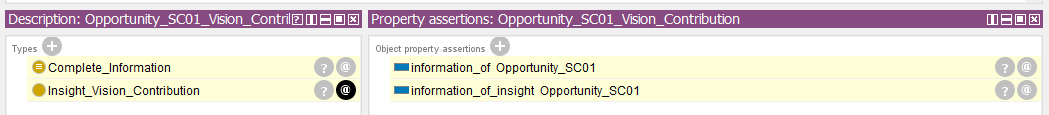
\includegraphics[width=17cm]{../../Images/05_Validation/05_RP_Opportunity_SC01_Vision_Contribution}
  \caption{The individual $Opportunity\_SC01\_Vision\_Contribution$ in Prot\'eg\'e. The $in{\f}ormation\_o{\f}$ object property is the inverse of the $has\_in{\f}ormation$ object property. The reasoner uses this characteristic to infer the $in{\f}ormation\_o{\f}$ object property. }
  \label{fig:RP_SC0_Opportunity_SC01_Vision_Contribution}
\end{figure}

We expect $4$ structural violations in scenario $SC0$.

\paragraph{Scenario 1 ($SC1$): Decision ontology pattern}
The information in the first scenario is complete, reproducible, meets the minimum level of consensus, and does not exceed the maximum level of conflict. Figure \ref{fig:RP_SC1_Vision} presents $Vision\_SC1$ as an example. $Vision\_SC1$ is complete based on the $has\_in{\f}ormation\_vision\_current\_state$, $*\_vision\_statement$, $*\_vision\_target\_condition$, and $*\_vision\_measurable\_objective$ object properties.

\begin{figure}[H]
\centering
  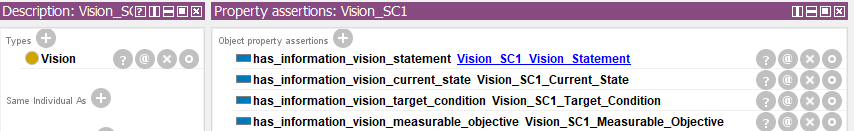
\includegraphics[width=17cm]{../../Images/05_Validation/05_RP_SC1_Vision_SC1.png}
  \caption{The individual $Vision\_SC1$ in Prot\'eg\'e. The reasoner infers the $based\_on\_evidence$ object property based on the $agrees\_with$ object property between $Stakeholder\_Value\_SC1$ and $Stakeholder\_Experience\_SC1$.}
  \label{fig:RP_SC1_Vision}
\end{figure}

The completeness pattern requires that each individual classified as $In{\f}ormation$ hosts the $data\_value$ and $data\_description$ data properties. Additionally, the vision statement should also include the $time\_{\f}rame$ data property. The reproducibility pattern requires that individuals classified as $In{\f}ormation$ are $based\_on\_evidence$ or $based\_on\_in{\f}ormation$. The conflict pattern requires that $In{\f}ormation$ individuals do not have conflicting evidence (represented by the object property $conflict\_with\_evidence$). Figure \ref{fig:RP_Vision_SC1_Statement} presents $Vision\_SC1\_Statement$ as an example of a complete and reproducible vision statement. $Vision\_SC1\_Statement$ meets the minimum consensus-level and does not have conflicting evidence.

\begin{figure}[H]
\centering
  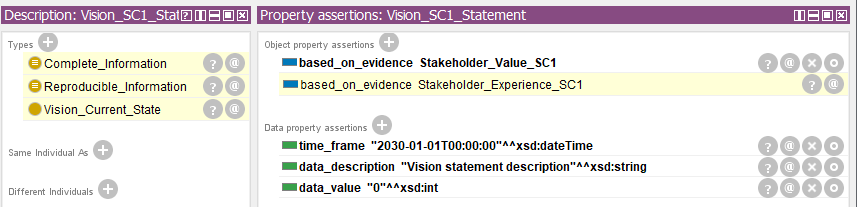
\includegraphics[width=17cm]{../../Images/05_Validation/05_RP_SC1_Vision_SC1_Statement.png}
  \caption{The individual $Vision\_SC1\_Statement$ in Prot\'eg\'e. The reasoner infers the $based\_on\_evidence$ object properties using the $agrees\_with$ object property between $Stakeholder\_Value\_SC1$ and $Stakeholder\_Experience\_SC1$.}
  \label{fig:RP_Vision_SC1_Statement}
\end{figure}

The consensus pattern requires that each individual classified as $Evidence$ agrees with at least one other evidence source. Figure \ref{fig:RP_Stakeholder_Value_SC1} presents $Stakeholder\_Value\_SC1$. $Stakeholder\_Value\_SC1$ agrees with $Stakeholder\_Experience\_SC1$. The reasoner infers that $Vision\_SC1\_Statement$ $based\_on\_evidence$ $Stakeholder\_Experience\_SC1$ from this. Figure \ref{fig:RP_Vision_SC1_Statement} presents the inferred object property.

\begin{figure}[H]
\centering
  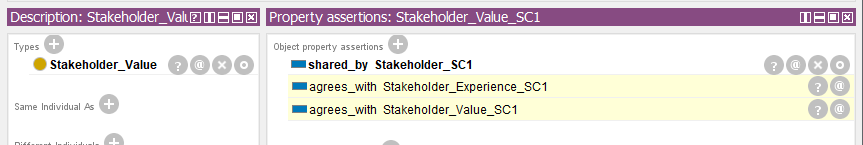
\includegraphics[width=17cm]{../../Images/05_Validation/05_RP_SC1_Stakeholder_Value_SC1.png}
  \caption{The individual $Stakeholder\_Value\_SC1$ in Prot\'eg\'e. $Stakeholder\_Value\_SC1$ agrees with $Stakeholder\_Experience\_SC1$. The reasoner infers that $Vision\_SC1\_Statement$ $based\_on\_evidence$ $Stakeholder\_Experience\_SC1$ from this.}
  \label{fig:RP_Stakeholder_Value_SC1}
\end{figure}

We expect $0$ violations of the completeness pattern in scenario $SC1$.

\paragraph{Scenario 2 ($SC2$): Completeness pattern}
In the second scenario, we attempt to detect incomplete information. We cannot reproduce missing information, and we cannot define a consensus or conflict-level for unreproducible information. As a result, the reproducibility, consensus, and conflict patterns are not relevant in this scenario.

We validate the completeness in two ways. The root classes need to have the specified object properties to the $In{\f}ormation$ classes, and the $In{\f}ormation$ classes need to have the data properties $data\_value$ and $data\_description$. Figure \ref{fig:RP_SC2_Completeness} presents a limited example of the root class $Challenge\_SC2$ and three of the related $In{\f}ormation$ classes. The $Challenge\_SC2\_Reach$ and $Challenge\_SC2\_Business\_Case$ are complete. However, the $Insight$ itself misses the $Insight\_Vision\_Contribution$ and $Challenge\_Frustration$. 

Additionally, $Challenge\_SC2\_Value$ misses the $data\_value$ and $data\_description$ data properties. We expect six violations related to $Challenge\_SC2$. Those six violations cover the missing $Challenge\_Frustration$, $Insight\_Vision\_Contribution$, and their related $data\_value$ and $data\_description$. Additionally, we expect and two violations related to $Challenge\_SC2\_Value$.

\begin{figure}[H]
\centering
  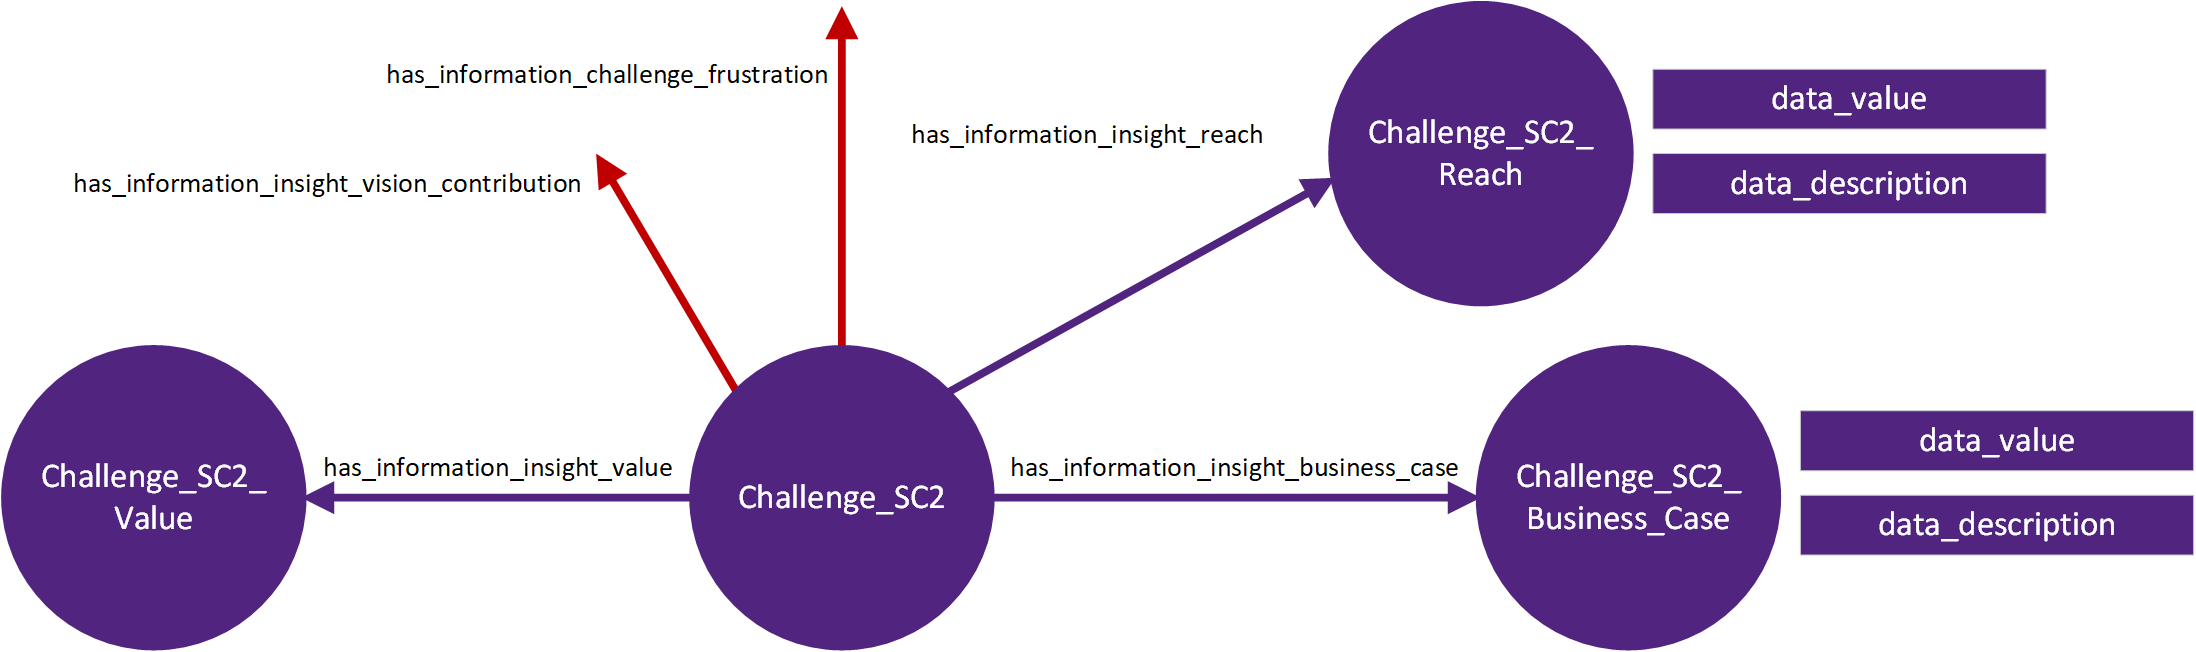
\includegraphics[width=17cm]{../../Images/05_Validation/05_RP_SC2_Completeness.png}
  \caption{An incomplete example of the root class $Insight$ and three of the related $In{\f}ormation$ classes.}
  \label{fig:RP_SC2_Completeness}
\end{figure}

Figure \ref{fig:RP_SC2_Challenge_SC2} presents $Challenge\_SC2$ in Prot\'eg\'e. The reasoner infers the $Addressed\_Challenge$ type from the $addressed\_by$ object property and infers the $has\_in{\f}ormation$ object properties from the specific $has\_in{\f}ormation\_$ object properties. For example, the reasoner infers $has\_information$ $Challenge\_SC2\_Value$ from $has\_in{\f}ormation\_insight\_value$ $Challenge\_SC2\_Value$.

\begin{figure}[H]
\centering
  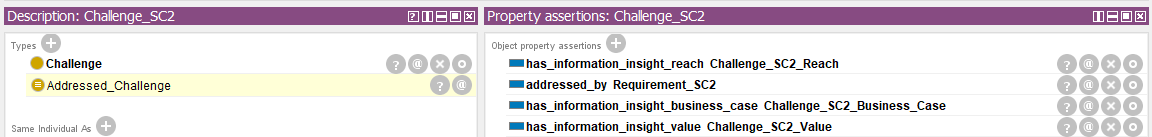
\includegraphics[width=17cm]{../../Images/05_Validation/05_RP_SC2_Challenge_SC2.png}
  \caption{The individual $Challenge\_SC2$ in Prot\'eg\'e. The reasoner infers the $Addressed\_Challenge$ type from the $addressed\_by$ object property and infers the $has\_in{\f}ormation$ object properties from the specific $has\_in{\f}ormation\_$ object properties.}
  \label{fig:RP_SC2_Challenge_SC2}
\end{figure}

We defined $Opportunity\_SC2$, $Requirement\_SC2$, and $Vision\_SC2$ as partially incomplete individuals. 

$Opportunity\_SC2$ refers to $2$ out of the $5$ individuals that store information. The $3$ missing individuals should generate $3$ violations each. Out of these $3$ individuals, $1$ is complete considering the $data\_value$ and $data\_description$. We expect $Opportunity\_SC2$ to trigger $(3*3)+(1*2)=11$ violations. 

$Requirement\_SC2$ refers to $4$ out of the $10$ individuals that store information. The $6$ missing individuals should generate $3$ violations each. Out of these $3$ individuals, $2$ are complete considering the $data\_value$ and $data\_description$. We expect $Requirement\_SC2$ to trigger $(6*3)+(2*2)=22$ violations. 

$Vision\_SC2$ refers to $1$ out of the $4$ individuals that store information. The measurable objective is among the missing $3$ individuals. The measurable objective should generate $4$ violations: $1$ for the individual itself, $1$ for the missing $data\_value$, $1$ for the missing $data\_description$, and $1$ for the missing $time\_{\f}rame$. The other missing individuals should generate $3$ violations each. The individuals are complete considering the $data\_value$ and $data\_description$. We expect $Vision\_SC2$ to trigger $4+(2*3)+(0*2)=10$ violations. 

We expect $43$ violations of the completeness pattern in scenario $SC2$.

\paragraph{Scenario 3 ($SC3$): Reproducibility}
Scenario $SC3$ contains information that is complete and unreproducible. We cannot define the consensus and conflict-level when information is not reproducible. As a result, the consensus and conflict patterns are not relevant in this scenario. 

We create $23$ individuals that are not reproducible. These individuals are not evidence-based and are not related to $In{\f}ormation$ using the $based\_on\_information$ object property. For example, $Requirement\_SC3\_Value$ contains the $data\_value$ and $data\_description$ data properties. Therefore, $Requirement\_SC3\_Value$ is complete. However, $Requirement\_SC3\_Value$ is not related to evidence or information. We expect $1$ violation related to $Requirement\_SC3\_Value$. Figure \ref{fig:RP_SC4_Requirement_SC3_Value} presents $Requirement\_SC3\_Value$ in Prot\'eg\'e.

\begin{figure}[H]
\centering
  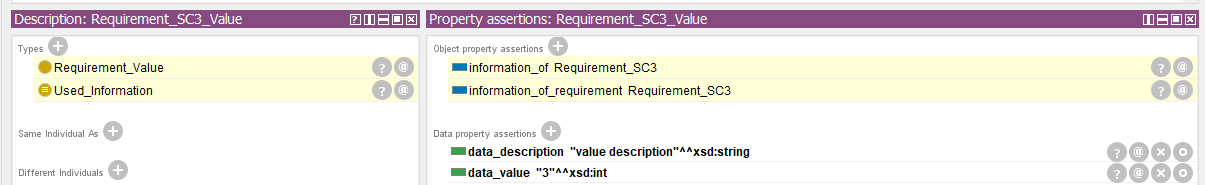
\includegraphics[width=17cm]{../../Images/05_Validation/05_RP_SC3_Requirement_SC3_Value.png}
  \caption{The individual $Requirement\_SC3\_Value$ in Prot\'eg\'e. The $in{\f}ormation\_o{\f}$ object property is the inverse of the $based\_on\_information$ object property. $Requirement\_SC3$ is based on $Requirement\_SC3\_Value$. The reasoner infers the $in{\f}ormation\_o{\f}$ from its inverse.}
  \label{fig:RP_SC4_Requirement_SC3_Value}
\end{figure}

We define $4$ root individuals for which we validate the reproducibility: $Opportunity\_SC3$, $Challenge\_SC3$, $Requirement\_SC3$, and $Vision\_SC3$. $Opportunity\_SC3$ requires $3$ knowledge criteria, $Challenge\_SC3$ requires $3$ knowledge criteria as well, and $Requirement\_SC3$ requires $4$ knowledge criteria. We base these $10$ knowledge criteria on another $13$ information sources spread out over $Opportunity\_SC3$, $Challenge\_SC3$, $Requirement\_SC3$, and $Vision\_SC3$. As a result, we expect $23$ violations of the reproducibility pattern in scenario $SC3$.

\paragraph{Scenario 4 ($SC4$): Conflict pattern}
In scenario $SC4$, we validate that the information is complete, reproducible, and does not cause any conflict. Figure \ref{fig:RP_SC4_Conflict} presents how this evidence disagrees with each other. Figure \ref{fig:RP_SC4_Stakeholder_Experience_SC4} presents $Stakeholder\_Experience\_SC4$ in Prot\'eg\'e.

\begin{figure}[H]
\centering
  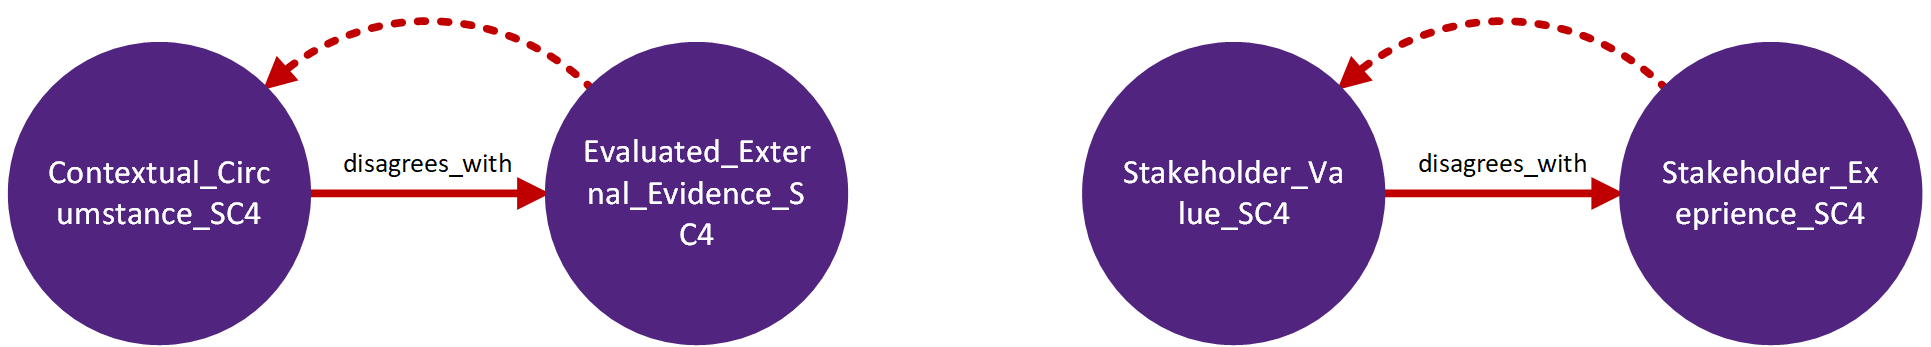
\includegraphics[width=15cm]{../../Images/05_Validation/05_SC4_Conflict_Inference.png}
  \caption{$4$ evidence sources disagree with each other. The fixed lines represent configured object properties. The dotted lines represent inferred object properties.}
  \label{fig:RP_SC4_Conflict}
\end{figure}

\begin{figure}[H]
\centering
  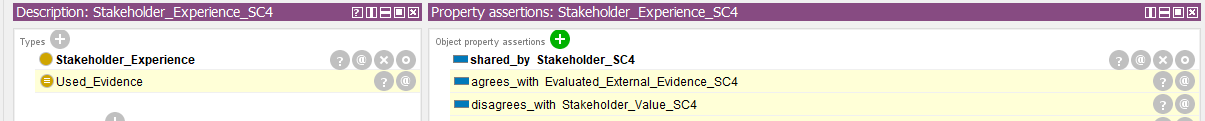
\includegraphics[width=17cm]{../../Images/05_Validation/05_RP_SC4_Stakeholder_Experience_SC4.png}
  \caption{The individual $Stakeholder\_Experience\_SC4$ in Prot\'eg\'e. The reasoner infers the $disagrees\_with$ object property using its symmetric and irreflexive characteristics.}
  \label{fig:RP_SC4_Stakeholder_Experience_SC4}
\end{figure}

For example, we use $Contextual\_Circumstance\_SC4$ as evidence for $Challenge\_SC4\_Business\_Case$. $Contextual\_Circumstance\_SC4$ disagrees with $Evaluated\_External\_Evidence\_SC4$. As a result, $Challenge\_SC4\_Business\_Case$ conflicts with these evidence sources. We expect $2$ violations related to $Challenge\_SC4\_Business\_Case$: $1$ for each evidence conflict. Figure \ref{fig:RP_SC4_Protege_Challenge_SC4_Business_Case} presents $Challenge\_SC4\_Business\_Case$ in Prot\'eg\'e.

\begin{figure}[H]
\centering
  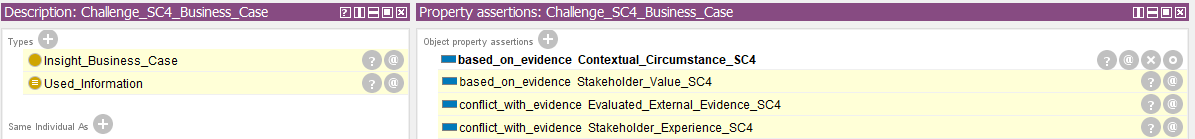
\includegraphics[width=17cm]{../../Images/05_Validation/05_RP_SC4_Challenge_SC4_Business_Case.png}
  \caption{The individual $Challenge\_SC4\_Business_Case$ in Prot\'eg\'e. The reasoner infers the $conflict\_with\_evidence$ object property from the super property figure \ref{fig:conflict_transitive} in section \ref{odp_conflict} \nameref{odp_conflict} presents.}
  \label{fig:RP_SC4_Protege_Challenge_SC4_Business_Case}
\end{figure}

We define $4$ conflicting evidence sources: $Contextual\_Circumstance\_SC4$, $Evaluated\_External\_Evidence\_SC4$ and $Stakeholder\_Value\_SC4$, $Stakeholder\_Experience\_SC4$\footnote{$Stakeholder\_Experience\_SC4$ and $Stakeholder\_Value\_SC4$ are shared by $Stakeholder\_SC4$ to ensure this evidence does not trigger any reproducibility violations.}. We based $16$ individuals on these evidence sources: $3$ individuals that host information for $Challenge\_SC4$, $3$ individuals that host information for $Opportunity\_SC4$, $6$ individuals that host information for, $Requirement\_SC4$, and another $4$ individuals that host information for $Vision\_SC4$. As a result, we expect $16$ violations of the conflict pattern in scenario $SC4$.

\paragraph{Scenario 5 ($SC5$): Consensus pattern}
The last scenario contains information that is complete and reproducible. It does not contain evidence conflicts. However, some information does not meet the defined consensus constraints. Each individual that the reasoner classifies as $Used\_Evidence$ should have at least one $agrees\_with$ object property to meet the consensus constraints. 

We have created $4$ evidence sources for scenario $SC5$: $Contextual\_Circumstance\_SC5$, $Evaluated\_External\_Evidence\_SC5$, $Stakeholder\_Experience\_SC5$, and $Stakeholder\_Value\_SC5$. These evidence sources serve as evidence for the $In{\f}ormation$ related to $SC5$, for example, $Opportunity\_SC5\_Reach$. $Stakeholder\_Experience\_SC5$ and $Stakeholder\_Value\_SC5$ agree with each other and should, therefore, not trigger any violations. Figure \ref{fig:05_RP_SC5_Stakeholder_Value_SC5} presents $Stakeholder\_Value\_SC5$ in Prot\'eg\'e.

\begin{figure}[H]
\centering
  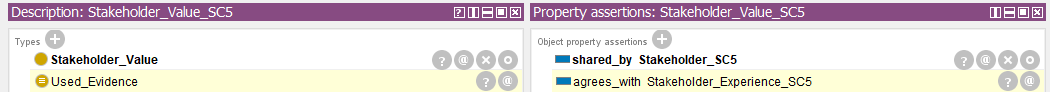
\includegraphics[width=17cm]{../../Images/05_Validation/05_RP_SC5_Stakeholder_Value_SC5.png}
  \caption{The $Stakeholder\_Value\_SC5$ in Prot\'eg\'e. The reasoner infers the $agrees\_with$ object property based its symmetric characteristic.}
  \label{fig:05_RP_SC5_Stakeholder_Value_SC5}
\end{figure}

Figure \ref{fig:05_RP_SC5_Evaluated_External_Evidence_SC5} presents, for example, $Evaluated\_External\_Evidence\_SC5$ in Prot\'eg\'e. $Evaluated\_External\_Evidence\_SC5$ is used as evidence for $Requirement\_SC5\_Increase\_Revenue$ and is, therefore, classified as $Used\_Evidence$. However, it does not have an $agrees\_with$ object property and should generate $1$ violation. $Contextual\_Circumstance\_SC5$ does not have an $agrees\_with$ and should generate $1$ violation as well.

\begin{figure}[H]
\centering
  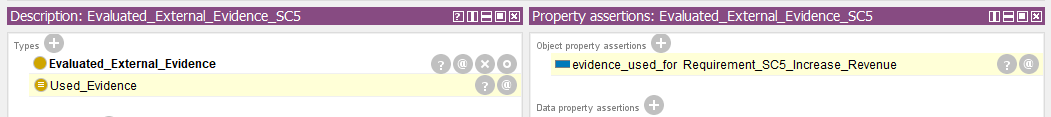
\includegraphics[width=17cm]{../../Images/05_Validation/05_RP_SC5_Evaluated_External_Evidence_SC5.png}
  \caption{The $Evaluated\_External\_Evidence\_SC5$ in Prot\'eg\'e. The $evidence\_used\_{\f}or$ object property is the inverse of the $based\_on\_evidence$ object property. The reasoner uses this inverse characteristic to infer the $evidence\_used\_{\f}or$ object property.}
  \label{fig:05_RP_SC5_Evaluated_External_Evidence_SC5}
\end{figure}

As a result, we expected $2$ violations of the consensus pattern in scenario $SC5$.

\paragraph{The result of the test scenarios}
Table \ref{table:rp_number_of_violations} presents the results of the tests. We detect $88$ violations. Figure \ref{fig:RP_SC_Results} presents an extract of the results as the SHACL4P plugin presents them in Prot\'eg\'e.

\begin{table}[H]
\centering
\caption{The number of expected and detected violations per scenario and pattern.}
\begin{tabular}{| p{3cm} | p{3cm} | p{4cm} | p{4cm} | }
\hline
\rowcolor{document}
\color{documentText}Scenario & \color{documentText}Scenario & \color{documentText}Expected violations & \color{documentText}Detected violations  \\
\hline
$SC0$ & Structural & 4 & 4 \\
\hdashline
$SC1$ & n/a & 0 & 0 \\
\hdashline
$SC2$ & Completeness & 43 & 43 \\
\hdashline
$SC3$ & Reproducibility & 23 & 23 \\
\hdashline
$SC4$ & Conflict & 16 & 16 \\
\hdashline
$SC5$ & Consensus & 2 & 2 \\
\hline
\end{tabular}
\label{table:rp_number_of_violations}
\end{table}

\begin{figure}[H]
\centering
  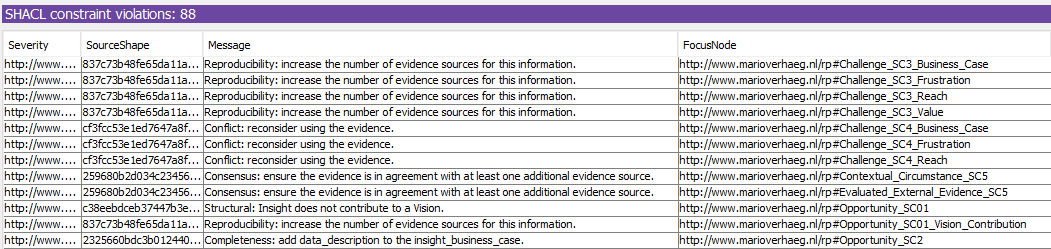
\includegraphics[width=17cm]{../../Images/05_Validation/05_RP_SC_Results.png}
  \caption{An extract of the results as the SHACL4P plugin presents them in Prot\'eg\'e.}
  \label{fig:RP_SC_Results}
\end{figure}

\subsubsection{Decision-relevant root individuals}
We determine the decision root individual that are relevant for a specific requirements prioritisation decision. The requirement prioritisation decision requires two individuals that are both classified as $Requirement$: $r_1$ and $r_2$. We know that a requirement needs to address an insight and that an insight has two sub-classes: opportunity and challenge. We also know that a vision should reproduce an insight. Code sample \ref{SPARQL_RP_VAL_Related} presents a SPARQL query that retrieves all opportunities, challenges, and visions related to a requirement using parameters $<r1>$ and $<r2>$. We execute the SPARQL query and feed the results into the set $RI$. We define function $rpri(r_1,r_2) = RI$ to logically represent the SPARQL query. We manually add $r_1$ and $r_2$ to $RI$.

\begin{lstlisting}[float,language=SPARQL1,caption={The first part of the SPARQL query gathers the insight(s) related to the specified requirements based on the $addresses$ object property: a $Requirement$ $addresses$ an insight. The second part of the SPARQL query gathers the vision(s) related to the specified requirements based on the $addresses$, $has\_in{\f}ormation$, and $based\_on\_in{\f}ormation$ object properties.},label={SPARQL_RP_VAL_Related}][H]
SELECT DISTINCT ?ri 
WHERE 
{
	# Gather insights (opportunities and challenges)
	{
		?req rp:addresses ?ri .
		?ri rdf:type ?t
		FILTER(?t != owl:Thing && ?t != rp:Addressed_Insight &&	?t != rp:Addressed_Opportunity && ?t != rp:Addressed_Challenge && ?t != rp:Insight).
	}
	UNION
	# Gather visions
	{
		?req rp:addresses ?ins .
		?ins rp:has_information ?ivc .
		?ivc rdf:type rp:Insight_Vision_Contribution .
		?ivc rp:based_on_information ?vcs .
		?ri rp:has_information ?vcs .
		?ri rdf:type ?t .	
		FILTER(?t != owl:Thing).				
	}
	FILTER(?req = <r1> || ?req = <r2>)
}
\end{lstlisting}

\subsubsection{Test scenarios for the decision presentation pattern}
We use four requirements to validate the decision presentation pattern. Each requirement has a different information maturity-level. The software product manager prioritises $Requirement\_SC1$ and $Requirement\_SC2$ in test scenario $DEC1$. The software product manager prioritises $Requirement\_SC3$ and $Requirement\_SC4$ in test scenario $DEC2$.

% ========================================================== DEC1 ===============================================================================================

\paragraph{Decision $DEC1$: $Requirement\_SC1$ versus $Requirement\_SC2$}
A software product manager needs to decide if $Requirement\_SC1$ is more important than $Requirement\_SC2$. The first question we ask is:

\begin{center}
\large\color{document}{Is the information ready for an evidence-based decision?}
\end{center}

The first dashboard of the decision presentation pattern helps the decision-maker to answer this question. We define the consolidated information maturity-level, and the evidence spread for these two requirements to generate this dashboard. 

We use function $rpri(Requirement\_SC1,Requirement\_SC2)$ to define $RI_{DEC1}$. $RI_{DEC1}$ is the set of decision-relevant root individuals. $RI_{DEC1}$ includes $Challenge\_SC1$, $Opportunity\_SC1$, $Challenge\_SC2$, $Opportunity\_SC2$, $Vision\_SC1$, and $Vision\_SC2$. We manually add $Requirement\_SC1$ and $Requirement\_SC2$ to $RI_{DEC1}$. Table \ref{table:rp_maximum_evidence_sc1} presents the maximum and the actual number of violations per decision-relevant root individual. We conclude that decision $DEC1$ can generate up to $239$ violations, and that decision $DEC1$ generates $52$ violations.

\begin{table}[H]
\centering
\caption{The maximum and the actual number of violations per decision-relevant root individual.}
\begin{tabular}{| p{3cm} | p{0.8cm} | p{0.8cm} | p{0.8cm} | p{0.8cm} | p{1.2cm} | p{0.8cm} | p{0.8cm} | p{0.8cm} | p{0.8cm} | p{1.2cm} |}
\hline
\rowcolor{document}
\color{documentText}Function & \color{documentText}$mvi_1$ & \color{documentText}$mvi_2$ & \color{documentText}$mvi_3$ & \color{documentText}$mvi_4$ & \color{documentText}$Total_{mv}$ & \color{documentText}$avi_1$ & \color{documentText}$avi_2$ & \color{documentText}$avi_3$ & \color{documentText}$avi_4$ & \color{documentText}$Total_{av}$ \\
\hline
$Requirement\_SC1$ 	& 30 & 10 & 2 & 10 & 52 & 0 & 0 & 0 & 0 & 0\\
\hdashline
$Challenge\_SC1$ 	& 15 & 5 & 2 & 5 & 27 & 0 & 0 & 0 & 0 & 0\\
\hdashline
$Opportunity\_SC1$ 	& 15 & 5 & 2 & 5 & 27 & 0 & 0 & 0 & 0 & 0\\
\hdashline
$Vision\_SC1$ 		& 14 & 4 & 2 & 4 & 24 & 0 & 0 & 0 & 0 & 0\\ 
\hdashline
$Requirement\_SC2$ 	& 30 & 10 & 4 & 10 & 54 & 23 & 0 & 0 & 0 & 22 \\ 
\hdashline
$Opportunity\_SC2$ 	& 15 & 5 & 4 & 5 & 29 & 11 & 0 & 0 & 0 & 11 \\ 
\hdashline
$Vision\_SC2$ 		& 14 & 4 & 4 & 4 & 26 & 10 & 0 & 0 & 0 & 10 \\
\hdashline
Total 				& 133 & 43 & 20 & 43 & 239 & 44 & 0 & 0 & 0 & 44 \\
\hline
\end{tabular}
\label{table:rp_maximum_evidence_sc1}
\end{table}

The information table \ref{table:rp_maximum_evidence_sc1} presents allows us to calculate the information maturity-level $iml$ for decision $DEC1$. Equation \ref{eq:information_maturity_level_SC1} shows that the information maturity-level for $DEC1$ is 82\%.

\begin{equation} \label{eq:information_maturity_level_SC1}
iml(RI) = \dfrac{mv_(RI)-av(RI)}{mv(RI)} = \dfrac{239-44}{239} = 0.816
\end{equation}

The first dashboard also presents the evidence spread. Table \ref{table:rp_evidence_spread_SC1} presents the evidence spread for decision $DEC1$ using the SPARQL query code sample \ref{SPARQL_ES} presents.

\begin{table}[H]
\centering
\caption{The evidence spread for the decision-relevant root individuals and the total evidence spread for this scenario.}
\begin{tabular}{| p{5cm} | p{4cm} |  p{4cm} |  p{2cm} | }
\hline
\rowcolor{document}
\color{documentText}Evidence &\color{documentText}$Requirement\_SC1$ & \color{documentText}$Requirement\_SC2$ & \color{documentText}Total \\
\hline
$Contextual\_Circumstance$ & 9 & 3 & 12 \\
\hdashline
$Stakeholder\_Value$ & 7 & 3 & 10 \\
\hdashline
$Evaluated\_External\_Evidence$ & 9 & 3 & 12 \\
\hdashline
$Stakeholder\_Experience$ & 7 & 3 & 10 \\
\hline
\end{tabular}
\label{table:rp_evidence_spread_SC1}
\end{table}

Figure \ref{fig:05_RP_Dashboard_Component_1_RP_SC1} presents a mock-up of the first decision presentation pattern dashboard. The dashboard reflects an information maturity-level of 82\% and the evidence spread table \ref{table:rp_evidence_spread_SC1} presents. The decision-maker needs to decide if the information maturity-level and evidence-spread are acceptable, depending on the impact of the decision.

\begin{figure}[H]
\centering
  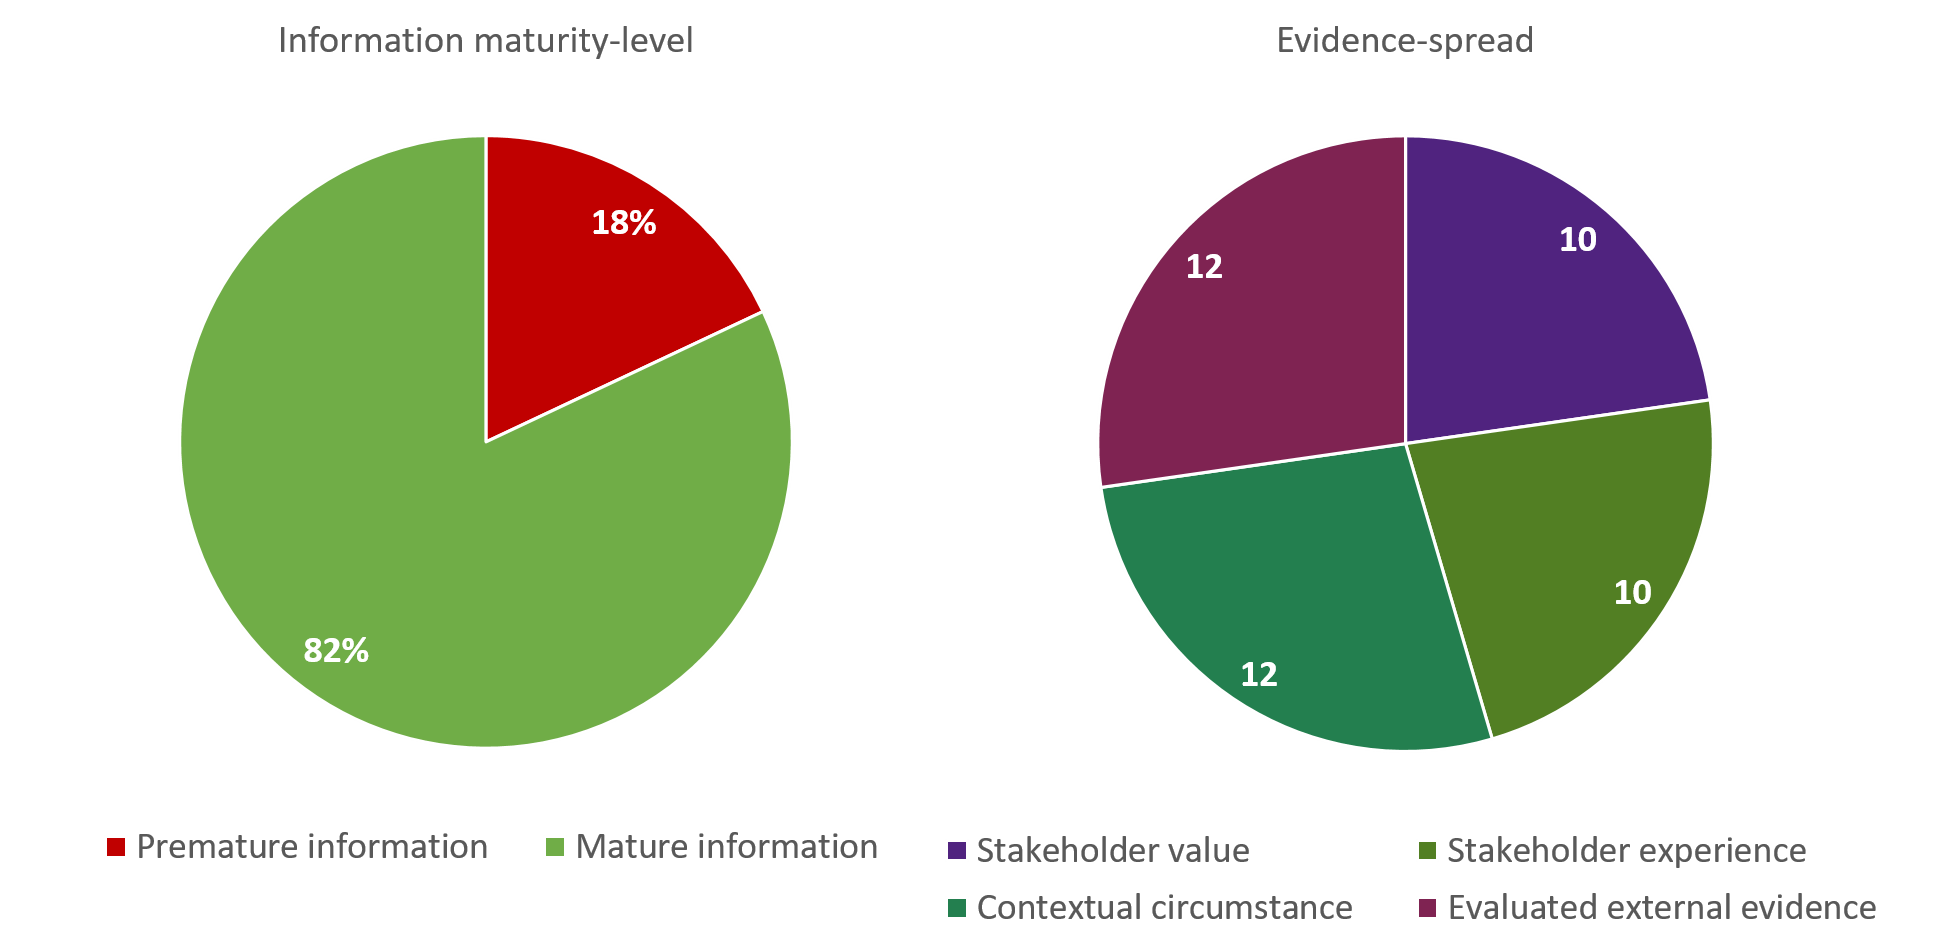
\includegraphics[width=14cm]{../../Images/05_Validation/05_RP_Dashboard_Component_1_RP_SC1.png}
  \caption{A mock-up of the first decision presentation pattern dashboard for decision $DEC1$. The dashboard reflects an information maturity-level of 82\% and the evidence spread table \ref{table:rp_evidence_spread_SC1} presents.}
  \label{fig:05_RP_Dashboard_Component_1_RP_SC1}
\end{figure}

The second dashboard of the decision presentation pattern presents the information maturity-level per pattern. We present the pattern-specific maximum and the actual violations in table \ref{table:rp_maximum_evidence_sc1}.

$Requirement\_SC1$ does not generate any completeness violations. $Requirement\_SC2$ generates $44$ completeness violations. The completeness pattern can generate up to $133$ violations in total for decision $DEC1$. $Requirement\_SC1$ and $Requirement\_SC2$ do not generate any other violations. 

Figure \ref{fig:05_RP_Dashboard_Component_2_RP_SC1} presents a mock-up of the second decision presentation pattern dashboard. The dashboard reflects the completeness maturity-level of $\dfrac{133-44}{133} = 0.669$, which results in 67\%. The maturity-levels of the other patterns are 100\% as they do not generate any violations.

\begin{figure}[H]
\centering
  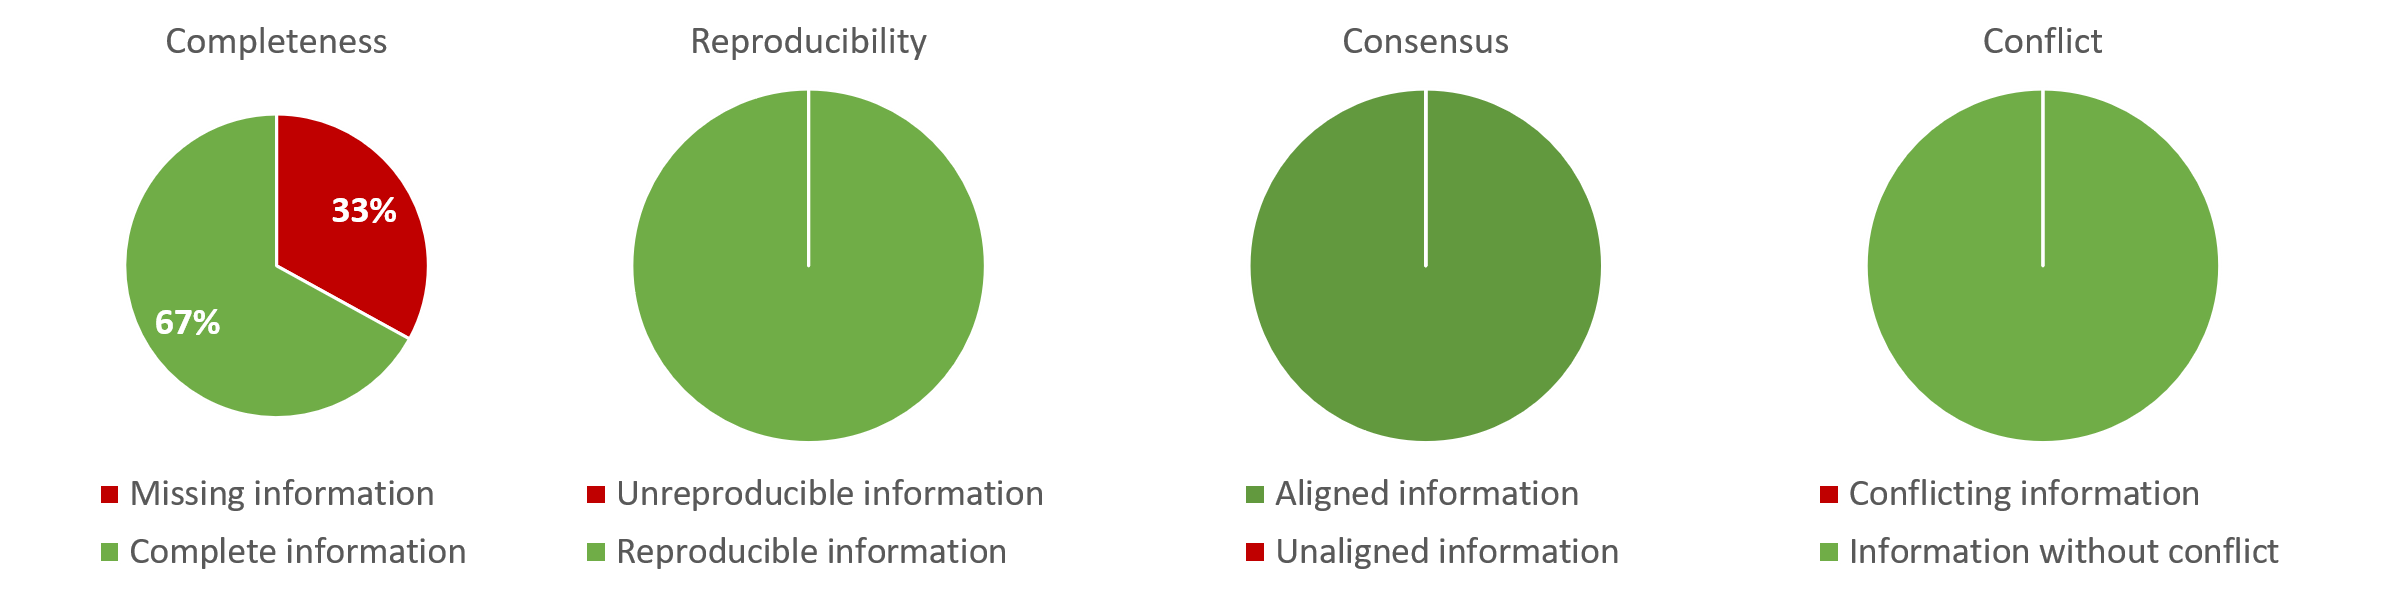
\includegraphics[width=17cm]{../../Images/05_Validation/05_RP_Dashboard_Component_2_RP_SC1.png}
  \caption{A mock-up of the second decision presentation pattern dashboard for decision $DEC1$. The dashboard reflects a completeness maturity-level of 67\%.}
  \label{fig:05_RP_Dashboard_Component_2_RP_SC1}
\end{figure}

To complete the missing information, the software product manager needs to know which information is incomplete. The third dashboard of the decision presentation pattern presents the completeness of information per decision-relevant individual.

Figure \ref{fig:05_RP_Dashboard_Component_3_RP_SC1_Completeness} presents a mock-up of the third decision presentation pattern dashboard, considering the software product manager selects $Opportunity\_SC2$. We observe that three decision-relevant individuals are incomplete. The bar charts give the software product manager an indication which individuals are causing the 67\% completeness maturity-level. The software product manager wants to know more information on a specific individual: $Opportunity\_SC2$. The dashboard presents the violations related to $Opportunity\_SC2$ in the table below the bar chart. We also observe the consolidation into root individuals: individuals classified as $Vision$, $Requirement$, $Opportunity$, or $Challenge$ are root individuals. The dashboard consolidates the violations of $Opportunity\_SC2\_Value$ under $Opportunity\_SC2$.

\begin{figure}[H]
\centering
  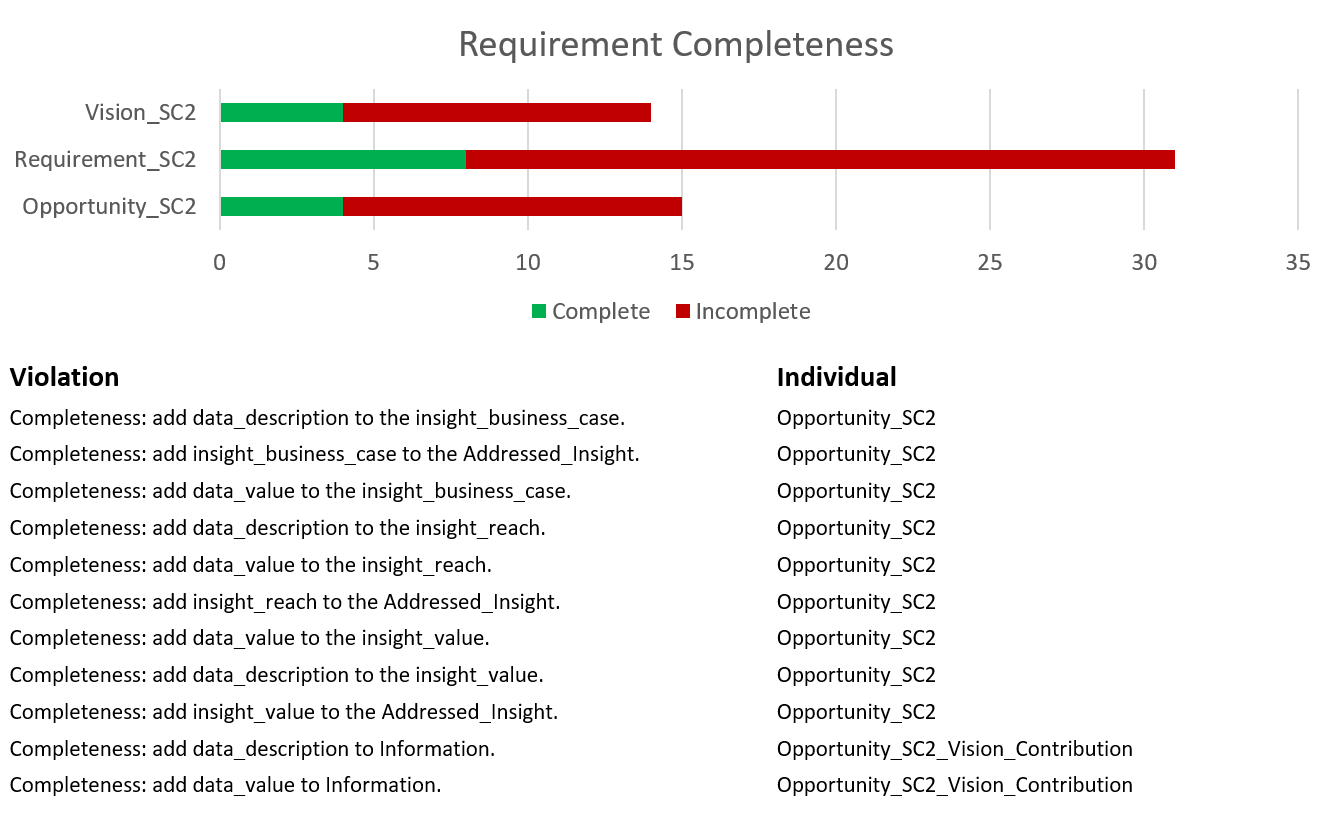
\includegraphics[width=16cm]{../../Images/05_Validation/05_RP_Dashboard_Component_3_RP_SC1_Completeness.png}
  \caption{A mock-up of the third decision presentation pattern dashboard, considering the decision-maker selected $Opportunity\_SC2$. We observe that four decision-relevant individuals are incomplete.}
  \label{fig:05_RP_Dashboard_Component_3_RP_SC1_Completeness}
\end{figure}

The software product manager wants to understand the reproducibility of the information. Figure \ref{fig:05_RP_Dashboard_Component_3_RP_SC1_Spread} presents the evidence spread using the third dashboard, considering the decision-maker clicked on the pie chart presenting the evidence spread in the first dashboard. This evidence spread does not violate any constraints. However, the software product manager can improve the evidence spread by elaborating on, for example, $Vision\_SC1$, which is based on two out of four evidence types.

\begin{figure}[H]
\centering
  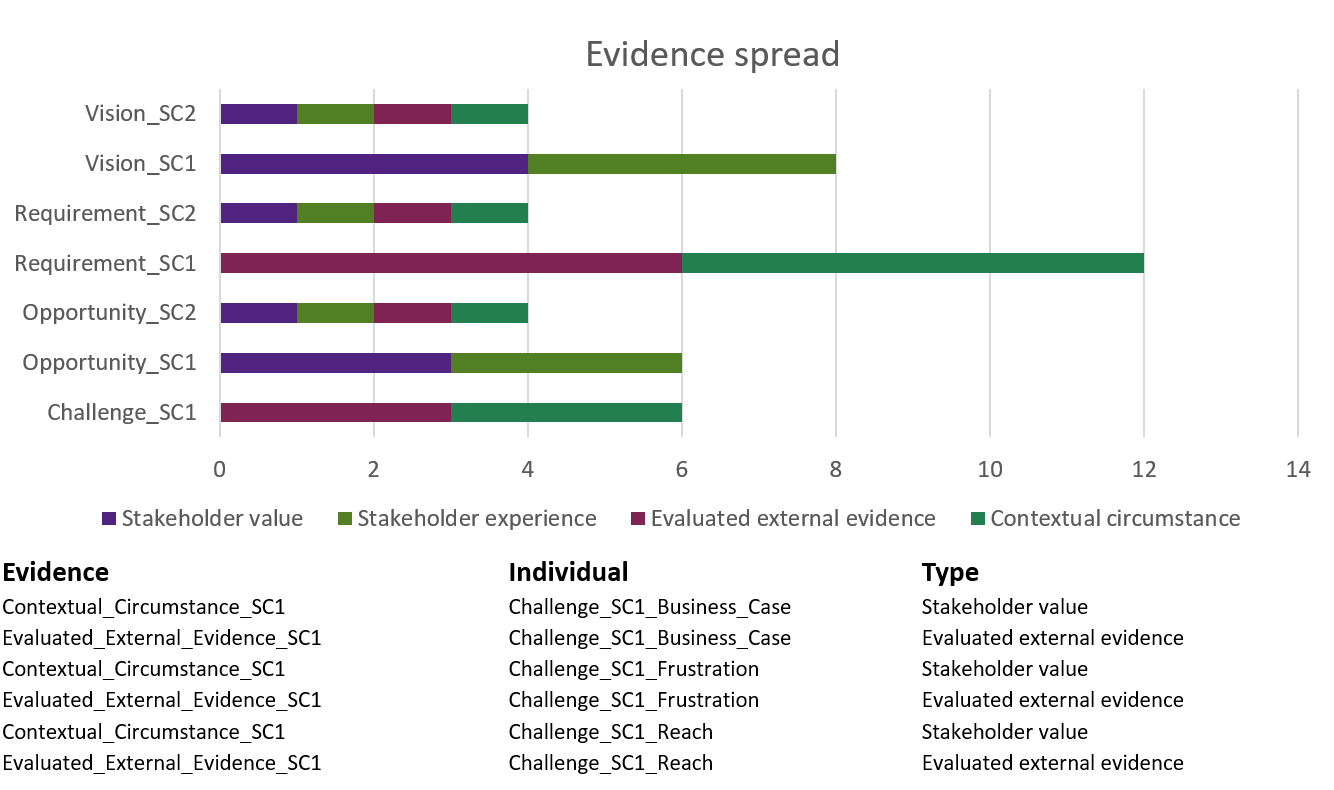
\includegraphics[width=16cm]{../../Images/05_Validation/05_RP_Dashboard_Component_3_RP_SC1_Spread.png}
  \caption{The evidence spread using the third dashboard, considering the decision-maker selected $Challenge\_SC1$. We observe that, for example, $Stakeholder\_Value$ and $Stakeholder\_Experience$ reproduce $Vision\_SC1$.}
  \label{fig:05_RP_Dashboard_Component_3_RP_SC1_Spread}
\end{figure}

% ========================================================== DEC2 ===============================================================================================

\paragraph{Decision $DEC2$: $Requirement\_SC3$ versus $Requirement\_SC4$}
A software product manager needs to decide if $Requirement\_SC3$ is more important than $Requirement\_SC4$. The first question we ask is:

\begin{center}
\large\color{document}{Is the information ready for this decision?}
\end{center}

The first decision presentation pattern dashboard helps a decision-maker to answer this question. We define the consolidated information maturity-level, and the evidence spread for the two requirements to generate this dashboard. 

We use function $rpri(Requirement\_SC3,Requirement\_SC4)$ to define $RI_{DEC2}$. $RI_{DEC2}$ is the set of decision-relevant root individuals. $RI_{DEC2}$ includes $Challenge\_SC3$, $Opportunity\_SC3$, $Challenge\_SC4$, $Opportunity\_SC4$, $Vision\_SC3$, and $Vision\_SC4$. We manually add $Requirement\_SC3$ and $Requirement\_SC4$ to $RI_{DEC2}$. Table \ref{table:rp_maximum_evidence_sc2} presents the maximum and the actual number of violations per decision-relevant root individual. The bottom line of the table presents the maximum and the actual number of violations per pattern. We conclude that decision $DEC2$ can generate up to $252$ violations. We conclude that decision $DEC2$ generates $37$ violations.

\begin{table}[H]
\centering
\caption{The maximum number of violations per decision-relevant root individual.}
\begin{tabular}{| p{3cm} | p{0.8cm} | p{0.8cm} | p{0.8cm} | p{0.8cm} | p{1.2cm} | p{0.8cm} | p{0.8cm} | p{0.8cm} | p{0.8cm} | p{1.2cm} |}
\hline
\rowcolor{document}
\color{documentText}Function & \color{documentText}$mvi_1$ & \color{documentText}$mvi_2$ & \color{documentText}$mvi_3$ & \color{documentText}$mvi_4$ & \color{documentText}$Total_{mv}$ & \color{documentText}$avi_1$ & \color{documentText}$avi_2$ & \color{documentText}$avi_3$ & \color{documentText}$avi_4$ & \color{documentText}$Total_{av}$ \\
\hline
$Requirement\_SC3$ 	& 30 & 10 & 0 & 10 & 50 & 0 & 9 & 0 & 0 & 9\\
\hdashline
$Challenge\_SC3$ 	& 15 & 5 & 0 & 5 & 25 & 0 & 4 & 0 & 0 & 4 \\
\hdashline
$Opportunity\_SC3$ 	& 15 & 5 & 0 & 5 & 25 & 0 & 4 & 0 & 0 & 4 \\
\hdashline
$Requirement\_SC4$ 	& 30 & 10 & 2 & 10 & 52 & 0 & 0 & 0 & 6 & 6 \\
\hdashline
$Challenge\_SC4$ 	& 15 & 5 & 2 & 5 & 27 & 0 & 0 & 0 & 3 & 3 \\ 
\hdashline
$Opportunity\_SC4$ 	& 15 & 5 & 2 & 5 & 27 & 0 & 0 & 0 & 3 & 3 \\ 
\hdashline
$Vision\_SC3$ 		& 14 & 4 & 0 & 4 & 22& 0 & 4 & 0 & 0 & 4 \\
\hdashline
$Vision\_SC4$ 		& 14 & 4 & 2 & 4 & 24 & 0 & 0 & 0 & 4 & 4 \\
\hdashline
Total 				& 148 & 48 & 8 & 48 & 252 & 0 & 21 & 0 & 16 & 37 \\
\hline
\end{tabular}
\label{table:rp_maximum_evidence_sc2}
\end{table}

The information presented in table \ref{table:rp_maximum_evidence_sc2} allows us to calculate the information maturity-level $iml$ for decision $DEC2$. Equation \ref{eq:information_maturity_level_SC2} shows that the information maturity-level for $DEC2$ is 85\%.

\begin{equation} \label{eq:information_maturity_level_SC2}
iml(RI) = \dfrac{mv_(RI)-av(RI)}{mv(RI)} = \dfrac{252-37}{252} = 0.853
\end{equation}

The first dashboard also presents the evidence spread. Table \ref{table:rp_evidence_spread_SC2} presents the evidence spread for decision $DEC2$ using the SPARQL query code sample \ref{SPARQL_ES} presents.

\begin{table}[H]
\centering
\caption{The evidence spread for the decision-relevant root individuals and the total evidence spread for this scenario.}
\begin{tabular}{| p{5cm} | p{4cm} |  p{4cm} |  p{2cm} | }
\hline
\rowcolor{document}
\color{documentText}Evidence &\color{documentText}$Requirement\_SC3$ & \color{documentText}$Requirement\_SC4$ & \color{documentText}Total \\
\hline
$Contextual\_Circumstance$ & 0 & 13 & 13 \\
\hdashline
$Stakeholder\_Value$ & 0 & 13 & 13 \\
\hdashline
$Evaluated\_External\_Evidence$ & 0 & 3 & 3 \\
\hdashline
$Stakeholder\_Experience$ & 0 & 3 & 3 \\
\hline
\end{tabular}
\label{table:rp_evidence_spread_SC2}
\end{table}

Figure \ref{fig:05_RP_Dashboard_Component_1_RP_SC2} presents a mock-up of the decision presentation pattern first dashboard. The dashboard reflects an information maturity-level of 85\% and the evidence spread table \ref{table:rp_evidence_spread_SC2} presents. The decision-maker needs to decide if the information maturity-level and evidence-spread are acceptable, depending on the impact of the decision.

\begin{figure}[H]
\centering
  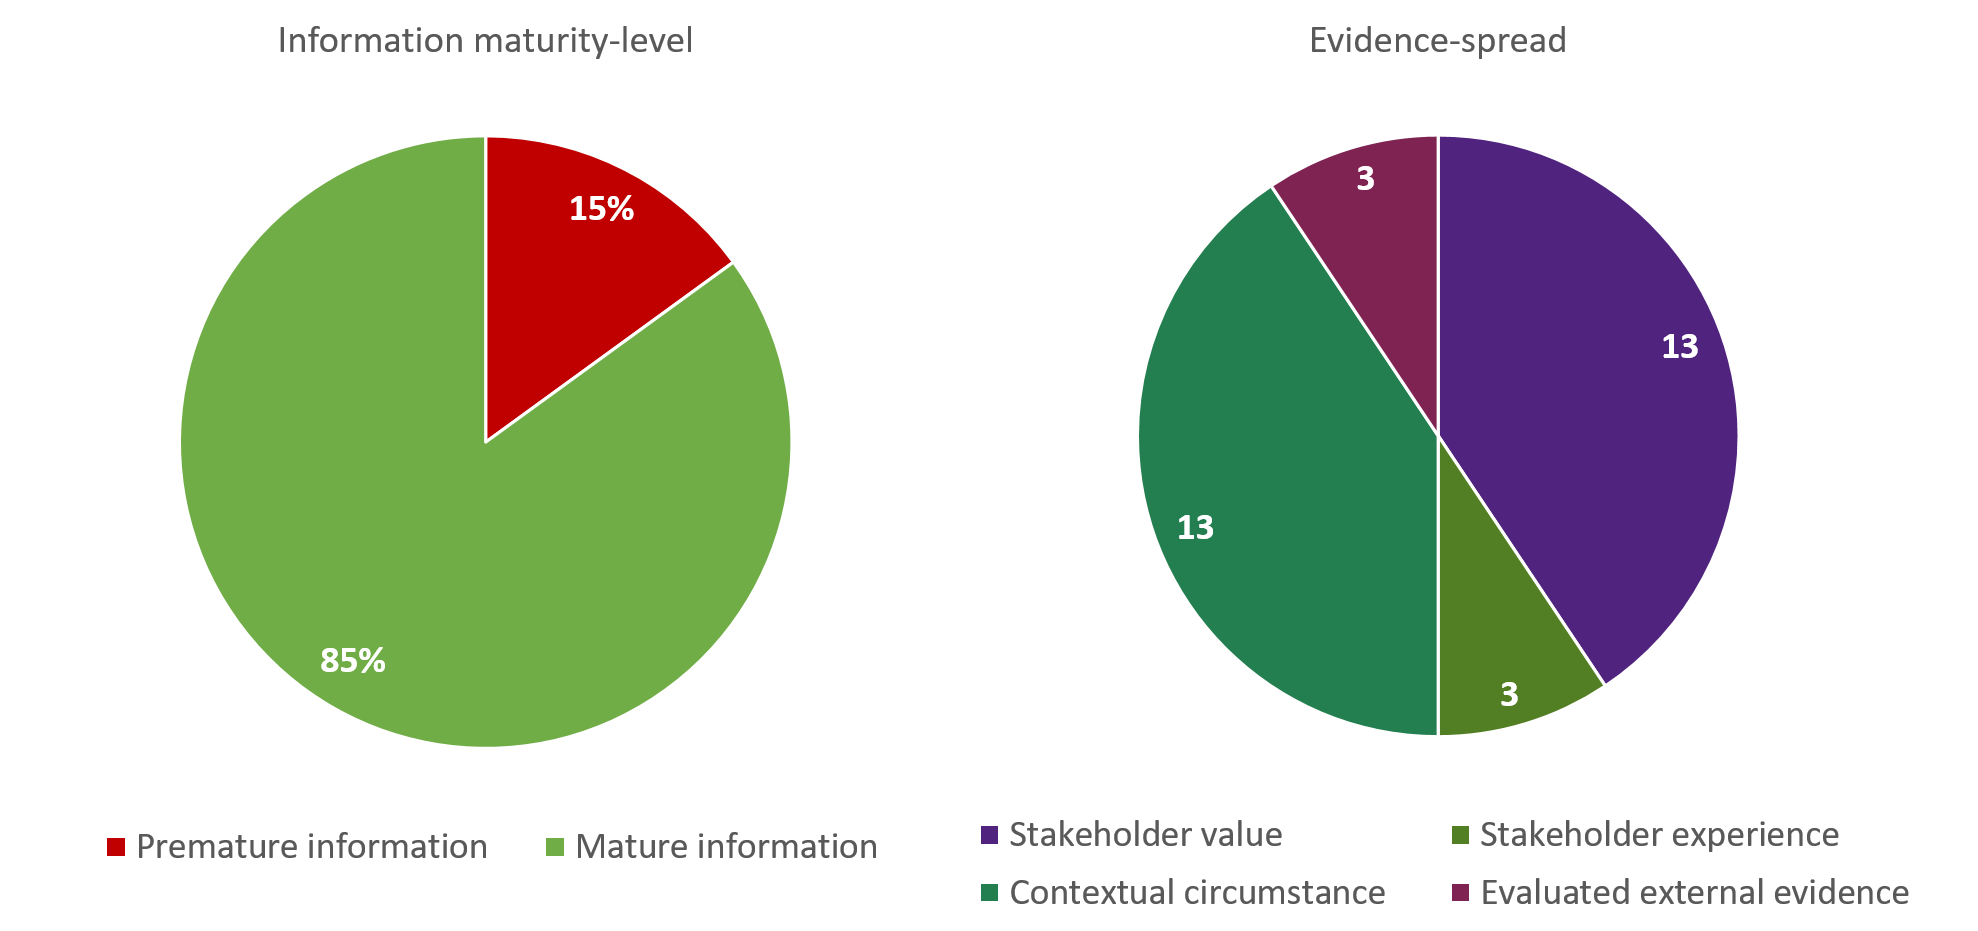
\includegraphics[width=14cm]{../../Images/05_Validation/05_RP_Dashboard_Component_1_RP_SC2.png}
  \caption{A mock-up of the first decision presentation pattern dashboard for test scenario $DEC2$. The dashboard reflects an information maturity-level of 85\% and the evidence spread table \ref{table:rp_evidence_spread_SC2} presents.}
  \label{fig:05_RP_Dashboard_Component_1_RP_SC2}
\end{figure}

The second decision presentation pattern dashboard presents the information maturity-level per pattern. We present the pattern-specific maximum and the actual violations in table \ref{table:rp_maximum_evidence_sc2}.

$Requirement\_SC3$ and $Requirement\_SC4$ do not generate any completeness violations. We use $Requirement\_SC3$ to test the reproducibility pattern, and it generates $21$ reproducibility violations. The reproducibility pattern can generate up to $48$ violations for decision $DEC2$. We use $Requirement\_SC4$ to test the conflict pattern, and it generates $16$ conflict violations. The conflict pattern can generate up to $48$ violations for decision $DEC2$. $Requirement\_SC3$ and $Requirement\_SC4$ do not generate any other violations. 

Figure \ref{fig:05_RP_Dashboard_Component_2_RP_SC2} presents a mock-up of the second decision presentation pattern dashboard. The dashboard reflects the reproducibility maturity-level of $\dfrac{48-21}{48} = 0.563$, which results in 56\% and the conflict maturity-level of $\dfrac{48-16}{48} = 0.667$, which results in 67\%. The maturity-levels of the other patterns are 100\% as they do not generate any violations.

\begin{figure}[H]
\centering
  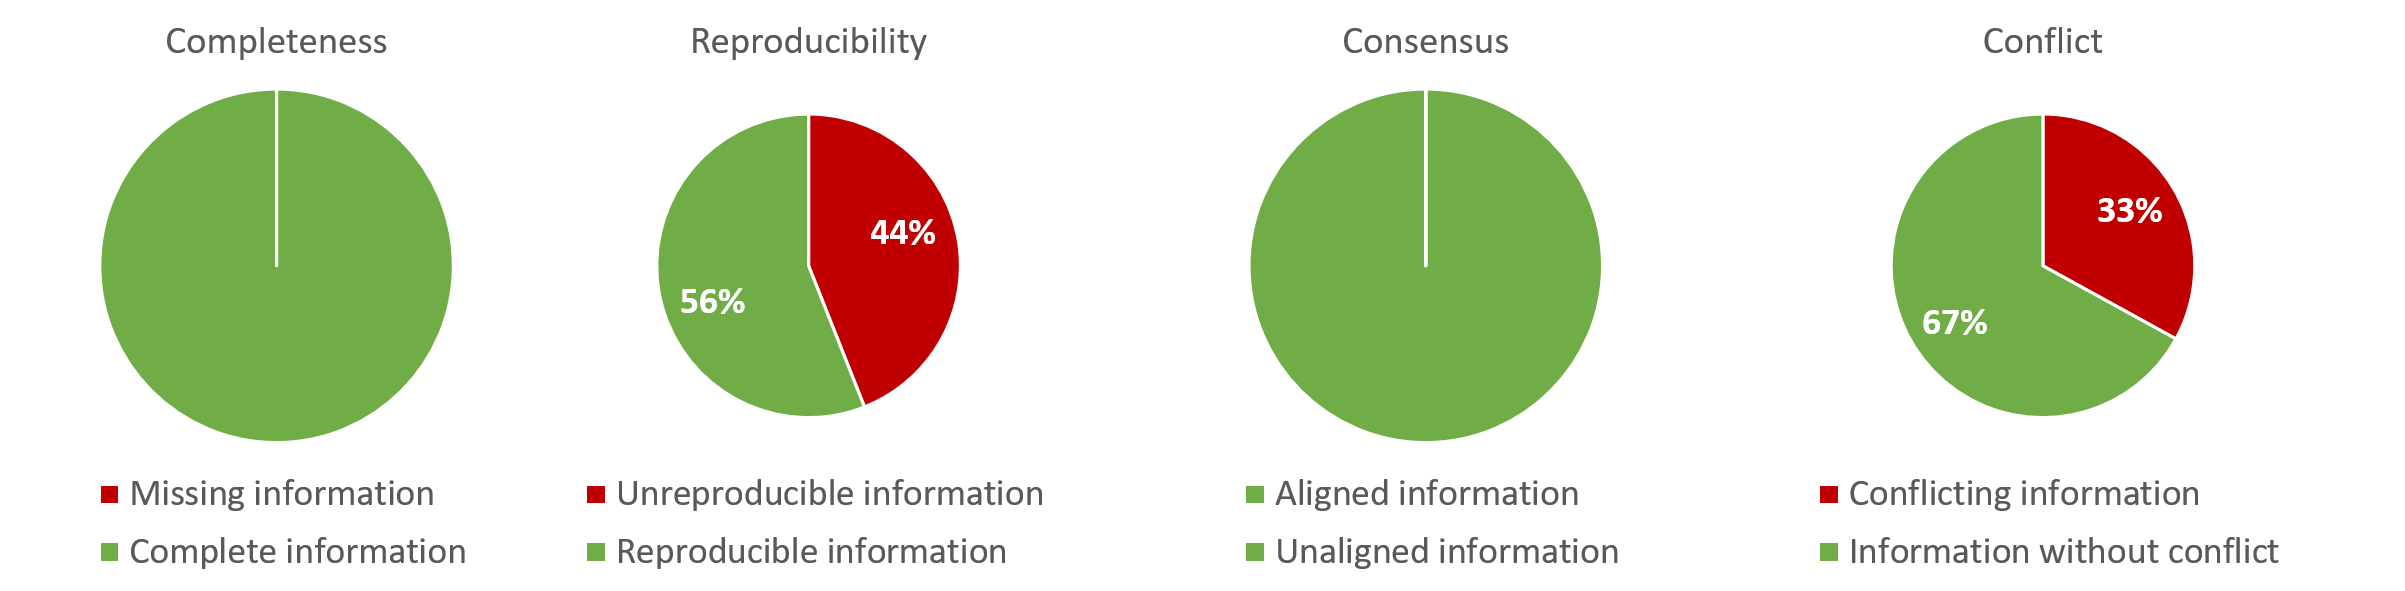
\includegraphics[width=17cm]{../../Images/05_Validation/05_RP_Dashboard_Component_2_RP_SC2.png}
  \caption{A mock-up of the second decision presentation pattern dashboard for decision $DEC2$. The dashboard reflects a reproducibility maturity-level of 56\% and a conflict maturity-level of 67\%.}
  \label{fig:05_RP_Dashboard_Component_2_RP_SC2}
\end{figure}

Figure \ref{fig:05_RP_Dashboard_Component_3_RP_SC2_Reproducibility} presents a mock-up of the third decision presentation pattern dashboard, considering the software product manager selected $Vision\_SC3$ and clicked on the pie chart presenting the reproducibility maturity-level in the second dashboard. We observe that four decision-relevant individuals are not reproducible. The bar charts give the software product manager an indication which individuals are causing the 57\% reproducibility maturity-level. The software product manager wants to know more information on a specific individual: $Vision\_SC3$. The dashboard presents the violations related to $Vision\_SC3$ in the table below the bar chart. We also observe the consolidation into root individuals: individuals classified as $Vision$, $Requirement$, $Opportunity$, or $Challenge$ are root individuals. 

\begin{figure}[H]
\centering
  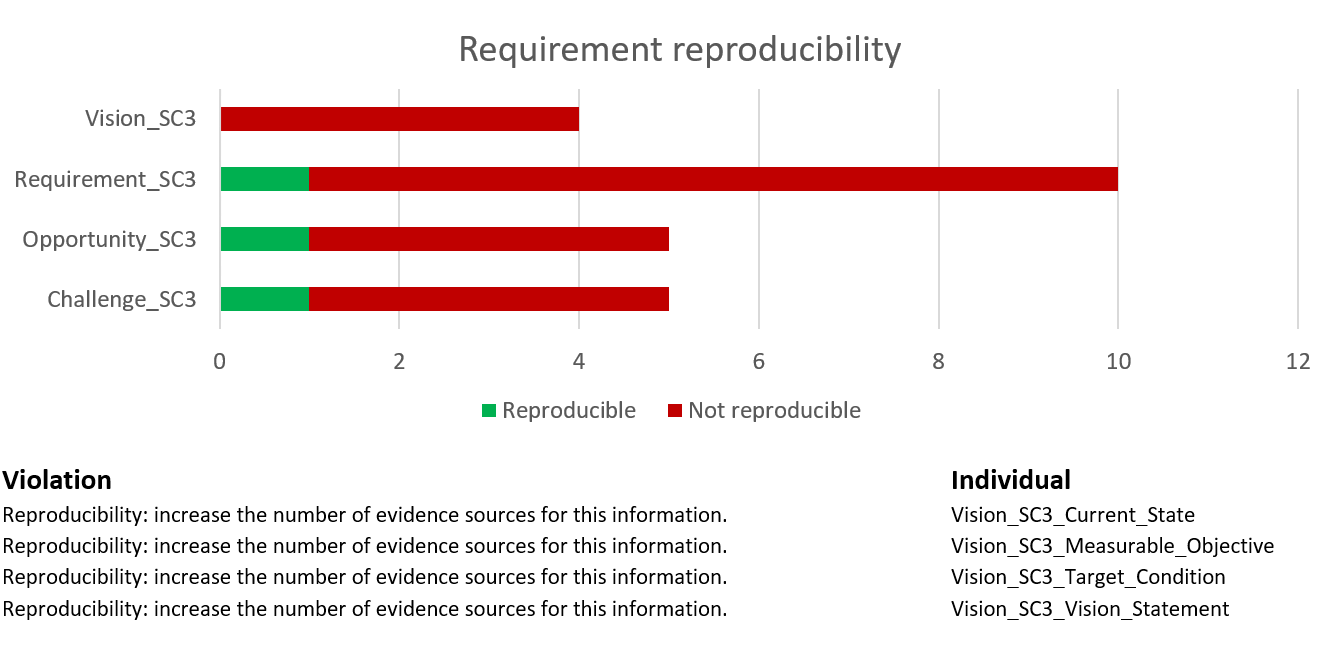
\includegraphics[width=16cm]{../../Images/05_Validation/05_RP_Dashboard_Component_3_RP_SC2_Reproducibility.png}
  \caption{A mock-up of the third decision presentation pattern dashboard, considering the decision-maker selected $Vision\_SC3$. We observe that four decision-relevant individuals are incomplete.}
  \label{fig:05_RP_Dashboard_Component_3_RP_SC2_Reproducibility}
\end{figure}

Figure \ref{fig:05_RP_Dashboard_Component_3_RP_SC2_Conflict} presents a mock-up of the third decision presentation pattern dashboard, considering the software product manager selected $Opportunity\_SC4$ and clicked on the pie chart presenting the conflict maturity-level in the second dashboard.

\begin{figure}[H]
\centering
  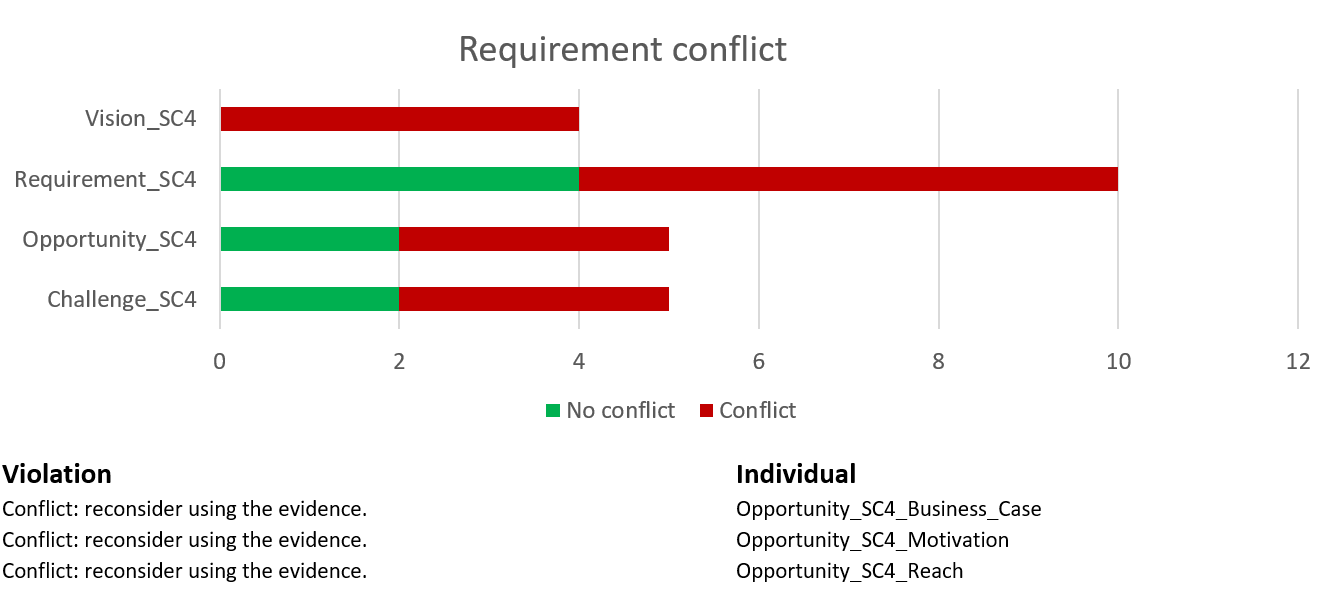
\includegraphics[width=16cm]{../../Images/05_Validation/05_RP_Dashboard_Component_3_RP_SC2_Conflict.png}
  \caption{A mock-up of the third decision presentation pattern dashboard, considering the decision-maker selected $Opportunity\_SC4$.}
  \label{fig:05_RP_Dashboard_Component_3_RP_SC2_Conflict}
\end{figure}

The software product manager wants to understand the reproducibility of the information. Figure \ref{fig:05_RP_Dashboard_Component_3_RP_SC2_Spread} presents the evidence spread using the third dashboard, considering the decision-maker clicked on the pie chart presenting the evidence spread in the first dashboard. 

\begin{figure}[H]
\centering
  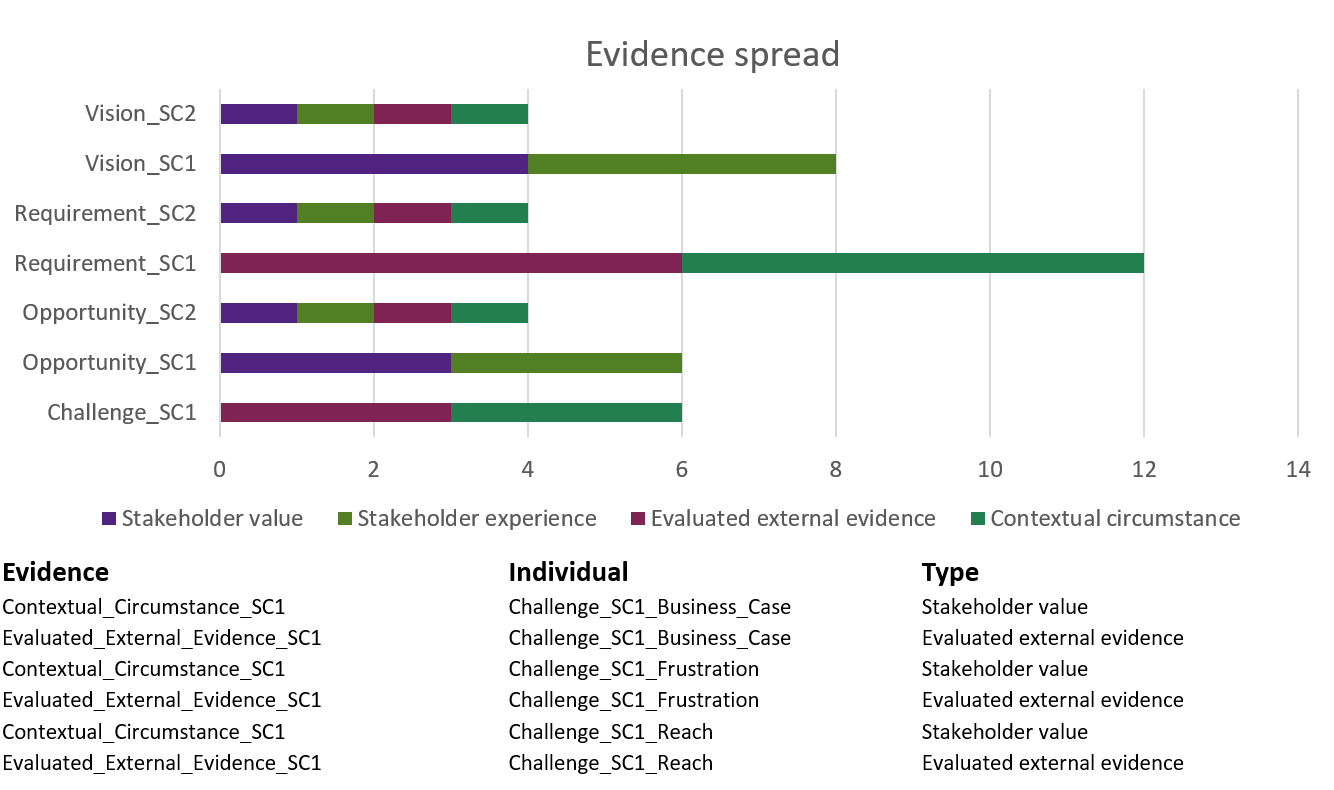
\includegraphics[width=16cm]{../../Images/05_Validation/05_RP_Dashboard_Component_3_RP_SC1_Spread.png}
  \caption{The evidence spread using the third dashboard.}
  \label{fig:05_RP_Dashboard_Component_3_RP_SC2_Spread}
\end{figure}